
\documentclass{common/hap}
\usepackage[utf8]{inputenc}
\usepackage[english]{babel}
\usepackage{listings}
\usepackage{url}
\usepackage{amsmath}
\usepackage{longtable}
\usepackage{booktabs}
\usepackage{pdflscape}
\usepackage[table]{xcolor}
\definecolor{tabhighlight}{HTML}{fff8c5}
\usepackage{paralist}
\usepackage{color}
\usepackage[usenames,dvipsnames]{xcolor}
\usepackage{theorem}
\usepackage{amsfonts}
\usepackage{amssymb}
\usepackage{bm}
\usepackage{tikz}
\usepackage{float}
\setlength{\headheight}{15.2pt}

%% WARNING!: use 'pdflatex' command to compile this file.

\def\Title{Retrieval-augmented clinical chatbot \\ for Spanish and Basque\\}
\def\ShortTitle{RAG clinical chatbot ES/EU}
\def\Authors{Iker Gutierrez Fandiño}
\def\TutorOne{Dr. Ander Barrena Madinabeitia}
\def\TutorTwo{Dr. Eneko Agirre Bengoa}
\def\Date{September 2026}

\def\AbstractEusk{Abstract in Basque.}
\def\AbstractEng{Abstract in English.}

%%%%%%% Don't touch the following lines
%%%%%%% Taken from MEANING style
\newcommand {\deltitle}{ \LARGE {\textbf{\Title}}}
\DocTitle{\ShortTitle}
\DocDate{\Date}

\addto\captionsbasque{%
  \renewcommand{\contentsname}{Contents}%
  \renewcommand{\listfigurename}{List of figures}%
  \renewcommand{\listtablename}{List of tables}%
}

\begin{document}
\begin{titlepage}
{ \center
  \begin{minipage}{\textwidth}
    \centering
      \vspace{-0.8cm}
    
\includegraphics[height=3cm]{common/ehuLogo}
    \vspace{0.8cm}
  \end{minipage}
}\\
\begin{minipage}[t][5.5cm][c]{\textwidth}
  \center
  \vspace{0.5cm}
  \deltitle
  \vspace{1cm}
{ \large \textbf{Author:} \Authors }\\
{ \large \textbf{First supervisor:} \TutorOne }\\
{ \large \textbf{Second supervisor:} \TutorTwo }\\
\end{minipage}\\
\vspace{1cm}
\begin{center}
%  \centering \textcolor{blue}{\Huge \textbf{hap/lap}}
  \resizebox{0.7\linewidth}{!}{ \textcolor{blue}{\texttt{hap/lap}}}
\end{center}

\vspace{0.8cm}
\begin{center}
  Hizkuntzaren Azterketa eta Prozesamendua\\Language Analysis and Processing\\
\vspace{0.8cm}
  {\Large \textbf{Master Thesis}}
\end{center}
\vspace{0.3cm}
\begin{center}
  \Date
\end{center}
\HRule \\[0.4cm]
{ \textbf{Departments}: Computer Systems and Languages, Computational Architectures and Technologies, Computational Science and Artificial Intelligence, Basque Language and Communication, Communications Engineer. }\\[0.4cm]
 \HRule \\[1.5cm]

\end{titlepage}
\renewcommand{\thepage}{\roman{page}}
\cleardoublepage
\newpage
\begin{center}
  \vspace*{\fill}
  \begin{minipage}{1.0\textwidth}
    \begin{center}
     \textbf{Laburpena}\\
     \AbstractEusk
    \end{center}
    \begin{center}
     \textbf{Abstract}\\
     \AbstractEng
    \end{center}
  \end{minipage}
  \vspace*{\fill}
\end{center}
\cleardoublepage
\tableofcontents
\cleardoublepage
\listoffigures
\cleardoublepage
\listoftables
\cleardoublepage
\setcounter{page}{1}
\renewcommand{\thepage}{\arabic{page}}
%%%%%%%%%%%%%%%%%%%%%%%%%%%%%%%%%%%%%%%%%%%%%%%%%%%%%%%%



%% ─────────────────────────────────────────────────────────────────────────────
\section{Project definition}
\label{sec:definition}

\subsection{Motivation}
\label{sec:motivation}

Clinical question answering in low-resource languages such as Basque (Euskera) remains largely unsolved.
Even for Spanish, the availability of biomedical language models and domain-specific benchmarks is limited compared to English.
This project builds and evaluates a retrieval-augmented generation (RAG) pipeline for clinical chatbot applications in both Spanish and Basque, targeting two complementary tasks: open-answer clinical questions drawn from the SNS1064 corpus, and multiple-choice medical exam questions from the CasiMédicos-Arg dataset \citep{sviridova-etal-2024-casimedicos}.

\subsection{Objectives}
\label{sec:objectives}

The main goal of this thesis is to determine which combination of retrieval strategy, language model, and inference-time reasoning technique yields the best performance on Spanish and Basque clinical question answering.
The specific objectives are:

\begin{compactenum}
  \item Design and implement an extractive-format RAG pipeline compatible with multiple generator models.
  \item Compare dense retrieval (multilingual E5) with cross-encoder reranking (multilingual MS MARCO) across different top-$k$ settings.
  \item Evaluate the effect of few-shot prompting (3-shot) combined with retrieval.
  \item Assess the benefit of self-feedback (a second LLM call that revises the initial answer) across all conditions.
  \item For Qwen3.5-9B, evaluate the additional effect of chain-of-thought thinking mode.
  \item Compare a general-purpose multilingual model (Mistral-7B-Instruct, Qwen3.5-9B) with a Basque-adapted model (Latxa-Llama-3.1-8B-Instruct) for Basque tasks.
\end{compactenum}

\subsection{Hypothesis}
\label{sec:hypothesis}

We hypothesise that combining dense retrieval with cross-encoder reranking and few-shot prompting will consistently outperform retrieval-free baselines, and that Basque-adapted models will outperform generic multilingual models on Basque clinical tasks despite a smaller parameter count.

%% ─────────────────────────────────────────────────────────────────────────────
\section{System description}
\label{sec:system}

\subsection{Retrieval pipeline}
\label{sec:retrieval}

Documents are indexed using FAISS with multilingual-E5-large embeddings.
At inference time the top-$k$ candidates are optionally re-ranked by a multilingual MS MARCO cross-encoder.
Retrieved passages are concatenated into the prompt context.

\subsection{Generation}
\label{sec:generation}

Three generator models are evaluated:
\textbf{Mistral-7B-Instruct-v0.3} (Spanish experiments),
\textbf{Qwen3.5-9B} (Spanish, with optional thinking mode), and
\textbf{Latxa-Llama-3.1-8B-Instruct} paired with \textbf{Llama-3.1-8B-Instruct} (Basque experiments).
All models use an extractive-format prompt that instructs the model to answer using only information present in the retrieved context.

\subsection{Self-feedback}
\label{sec:sf}

Self-feedback (SF) is a two-call procedure: the model first generates an answer, then receives a second prompt asking it to critique and revise that answer.
The revised answer is used for evaluation.

\subsection{Evaluation metrics}
\label{sec:metrics}

Answers are evaluated against gold references using:
ROUGE-L F1 (lexical overlap),
cosine similarity of multilingual-E5-large embeddings (semantic overlap), and
BERTScore F1 with \texttt{bert-base-multilingual-cased} (contextualised token matching).
All scores are reported as percentages out of 100.

%% ─────────────────────────────────────────────────────────────────────────────
\section{The SNS-1064 Dataset}
\label{sec:sns1064}

Question answering (QA) systems for the clinical domain require structured and high-quality data to support reliable retrieval and generation.
This section presents the SNS-1064 dataset, designed for RAG-based clinical QA tasks.
The dataset is derived from Spanish-language clinical guidebooks written by medical experts.
Clinical guidebooks consist of ``a set of recommendations based on a systematic review of the evidence and an assessment of the risks and benefits of different options, with the aim of optimizing patient care'' \citep{guiasalud}.

The main objective of this dataset is to transform unstructured clinical text into structured QA instances that separate questions, answers, evidence, and interpretative considerations.
This structure is intended to improve downstream retrieval and reasoning capabilities in clinical NLP systems.
The dataset and code are publicly available on GitHub: \url{https://github.com/iker-gutierrez/SNS-1064-dataset}.

\subsection{Dataset characteristics}
\label{sec:sns-characteristics}

\subsubsection{Qualitative description}

The dataset is constructed from 6 clinical guidebooks published by the SNS (\textit{Sistema Nacional de Salud} / Spanish National Health System).
Each guidebook covers a different clinical domain:

\begin{table}[H]
\centering
\small
\begin{tabular}{ll}
\toprule
\textbf{Guidebook} & \textbf{Source} \\
\midrule
Anxiety & \citet{ansiedad} \\
Diabetes & \citet{diabetes} \\
Ictus management & \citet{ictus} \\
Palliative care & \citet{paliativos} \\
Pediatric palliative care & \citet{paliativos_pediatria} \\
Secondary ictus prevention & \citet{prevencion_ictus} \\
\bottomrule
\end{tabular}
\caption{Clinical guidebooks included in the SNS-1064 dataset and their corresponding sources.}
\label{tab:sns-clinical-domains}
\end{table}

The dataset schema is presented in Table~\ref{tab:sns-schema}.
Each instance consists of a clinical question, an optional subquestion, a short judgement, supporting evidence extracted from the guideline, and optional interpretative considerations.
This structure enables a clear separation between answers (\textit{judgement} column) and their justification (\textit{evidence} and \textit{considerations} columns):

\begin{table}[H]
\centering
\small
\begin{tabular}{lll}
\toprule
\textbf{\#} & \textbf{Column} & \textbf{Description} \\
\midrule
0 & guidebook & File name of the guidebook \\
1 & topic & Clinical topic providing context \\
2 & question & Main clinical question \\
3 & subquestion & Refinement of the question (optional) \\
4 & judgement & Short answer to the \textit{(sub)question} \\
5 & evidence & Supporting scientific evidence \\
6 & considerations & Interpretative notes (optional) \\
\bottomrule
\end{tabular}
\caption{Schema of the SNS-1064 dataset.}
\label{tab:sns-schema}
\end{table}

For RAG-based systems, the columns of the dataset can be employed as follows:

\begin{itemize}
\item \textbf{Useful metadata}: guidebook.
\item \textbf{Model input}: topic, question, subquestion.
\item \textbf{Model output}: judgement, evidence, considerations.
\end{itemize}

\subsubsection{Quantitative description}

Table~\ref{tab:sns-totals} summarises the size of the dataset in terms of guidebooks, samples, sentences, and word tokens:

\begin{table}[H]
\centering
\begin{tabular}{lc}
\toprule
\textbf{Data type} & \textbf{Quantity} \\
\midrule
Clinical guidebooks & 6 \\
Samples & 1,064 \\
Sentences & 8,602 \\
Word tokens & 156,202 \\
\bottomrule
\end{tabular}
\caption{Total quantities of the SNS-1064 dataset.}
\label{tab:sns-totals}
\end{table}

Table~\ref{tab:sns-guidebook-dist} shows the distribution of samples across the six source guidebooks, illustrating the coverage of different clinical domains.

\begin{table}[H]
\centering
\begin{tabular}{lc}
\toprule
\textbf{Guidebook} & \textbf{Samples} \\
\midrule
Diabetes & 329 \\
Ictus management  & 254 \\
Anxiety & 248 \\
Palliative care & 111 \\
Secondary ictus prevention & 98 \\
Pediatric palliative care & 24 \\
\bottomrule
\end{tabular}
\caption{Number of samples per guidebook.}
\label{tab:sns-guidebook-dist}
\end{table}

In addition to global counts, per-feature statistics are reported in Table~\ref{tab:sns-length-stats}.
\textit{Questions} and \textit{subquestions} are relatively short (means of 10.2 and 8.5 tokens, respectively), while \textit{judgements} are even more concise on average (5.7 tokens), although they exhibit high variance.
In contrast, \textit{evidence} and \textit{considerations} are notably the longest, with mean lengths of 75.6 and 108.0 tokens and large standard deviations, indicating considerable variability.
This pattern reflects the structure of clinical guidelines, where concise questions and short answers are accompanied by detailed evidence-based explanations and extended interpretative notes.

\begin{table}[H]
\centering
\begin{tabular}{lcc}
\toprule
\textbf{Feature} & \textbf{Mean length} & \textbf{Std.\ dev.} \\
\midrule
question & 10.2 & 2.0 \\
subquestion & 8.4 & 3.2 \\
judgement & 3.9 & 7.0 \\
evidence & \textbf{73.2} & 126.3 \\
considerations & \textbf{85.8} & 187.6 \\
\bottomrule
\end{tabular}
\caption{Length statistics (in tokens) for each feature of the SNS-1064 dataset.}
\label{tab:sns-length-stats}
\end{table}

\subsection{Dataset construction pipeline}
\label{sec:sns-pipeline}

The dataset is generated using a rule-based Python pipeline that processes raw text and extracts structured text using regular expressions.
This approach has the advantage of being efficient (no GPU needed) and fully deterministic (no Machine Learning, no possible hallucinations).
Hallucinations can be especially harmful in the clinical domain.

An overview of the dataset construction pipeline is illustrated in Figure~\ref{fig:sns-pipeline}:

\begin{figure}[H]
\centering
\small
\resizebox{0.28\linewidth}{!}{
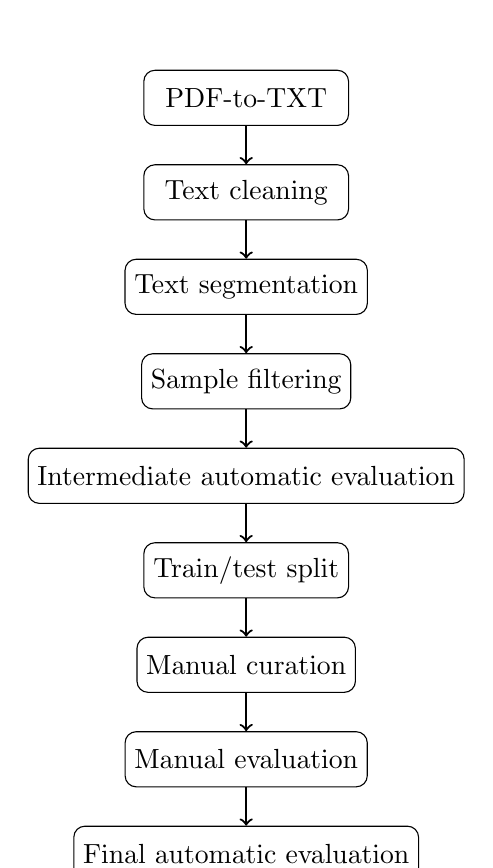
\begin{tikzpicture}[
    node distance=1.2cm,
    every node/.style={draw, rectangle, rounded corners, align=center, minimum width=2.6cm, minimum height=0.7cm},
    arrow/.style={->, thick}
]
\node (pdf) {PDF-to-TXT};
\node (clean) [below of=pdf] {Text cleaning};
\node (seg) [below of=clean] {Text segmentation};
\node (filter) [below of=seg] {Sample filtering};
\node (eval) [below of=filter] {Intermediate automatic evaluation};
\node (split) [below of=eval] {Train/test split};
\node (curation) [below of=split] {Manual curation};
\node (manualeval) [below of=curation] {Manual evaluation};
\node (finaleval) [below of=manualeval] {Final automatic evaluation};
\draw[arrow] (pdf) -- (clean);
\draw[arrow] (clean) -- (seg);
\draw[arrow] (seg) -- (filter);
\draw[arrow] (filter) -- (eval);
\draw[arrow] (eval) -- (split);
\draw[arrow] (split) -- (curation);
\draw[arrow] (curation) -- (manualeval);
\draw[arrow] (manualeval) -- (finaleval);
\end{tikzpicture}
}
\caption{Overview of the SNS-1064 dataset construction pipeline.}
\label{fig:sns-pipeline}
\end{figure}

\subsubsection{PDF-to-TXT}

PDF24 \citep{pdf24} was employed to convert each of the clinical guidebooks from PDF format into TXT format.
Although this introduces minor formatting noise (e.g.\ line breaks, headers, and pagination artifacts), these issues are addressed in the cleaning stage.

\subsubsection{Text cleaning}

Each line extracted from the TXT files is normalised using a dedicated cleaning function that performs the following operations:

\begin{itemize}
    \item Initial whitespace stripping.
    \item Bullet-like character removal: \{\textbullet{}, $\bullet$, \texttt{-}, \texttt{*}\}.
    \item Final whitespace stripping.
\end{itemize}

This step ensures that the text segmentation operates on uniform textual units, reducing noise introduced by PDF extraction artifacts.

\subsubsection{Text segmentation}

The core of the pipeline is a rule-based text segmentation built using regular expressions.
The text is processed sequentially, assigning each line to a structural component via pattern matching.
The segmentation logic is composed of the following patterns to identify input features (Table~\ref{tab:sns-input-triggers}) and output features (Table~\ref{tab:sns-output-triggers}):

\begin{table}[H]
\centering
\small
\begin{tabular}{l|l|c}
\toprule
\textbf{Input feature} & \textbf{Patterns} & \textbf{e.g.} \\
\midrule
\textit{topic} & After ``Pregunta'' \\
      & After ``Pregunta para responder'' \\
      & After ``Subpregunta'' \\
      & Before ``Contexto'' \\
\midrule
\textit{question} & \texttt{\textasciicircum[a-z])} & \texttt{a)}  \\
\midrule
\textit{subquestion} & \texttt{\textasciicircum[a-z]\textbackslash.\textbackslash d+\textbackslash.} & \texttt{a.1.} \\
\bottomrule
\end{tabular}
\caption{Text segmentation patterns for input features.}
\label{tab:sns-input-triggers}
\end{table}

\begin{table}[H]
\centering
\small
\begin{tabular}{l|l}
\toprule
\textbf{Output feature} & \textbf{Patterns} \\
\midrule
\textit{judgement} & After ``Juicio:'' \\
\midrule
\textit{evidence} & After ``Evidencia procedente de la investigaci\'{o}n:'' \\
\midrule
\textit{considerations} & After ``Consideraciones adicionales:'' \\
               & After ``Informaci\'{o}n adicional:'' \\
\bottomrule
\end{tabular}
\caption{Text segmentation patterns for output features.}
\label{tab:sns-output-triggers}
\end{table}

Input features are derived from header and pattern-based markers, which define sample boundaries and control when instances are flushed.
Output features are activated by keyword triggers and accumulate text until the trigger of the next feature.
This mechanism enables reconstruction of a hierarchical structure (\textit{topic} $\rightarrow$ \textit{question} $\rightarrow$ \textit{subquestion} $\rightarrow$ \textit{answers}) from flat text.

\subsubsection{Sample filtering}

After extraction, a filtering step was applied to remove noisy samples.
In particular, 70 instances in the dataset contain only placeholder references in the \textit{evidence} feature: \textit{Ver apartado anterior} (``See previous section'') or \textit{Ver apartados anteriores} (``See previous sections'').
These cases were removed because they do not provide any bibliographical source but instead refer to previous \textit{evidence} cells.
Keeping these placeholder instances would imply associating a single bibliographical source to several clinical questions, which may blur the semantic distance among different QA instances.
A short experiment confirms that RAG performance improves by 2.4\% when such instances are removed:

\begin{table}[H]
\centering
\begin{tabular}{lccc}
\toprule
\textbf{Data type} & \textbf{Unfiltered} & \textbf{Filtered} & \textbf{$\Delta$} \\
\midrule
judgement        & 84.5 & 85.3 & +0.8 \\
evidence         & 81.0 & 81.8 & +0.8 \\
considerations   & 79.7 & 85.2 & \textbf{+5.5} \\
overall & 81.7 & 84.1 & \textbf{+2.4} \\
\bottomrule
\end{tabular}
\caption{Cosine similarity (F1) results with and without sample filtering.}
\label{tab:sns-cosine-results}
\end{table}

\subsubsection{Intermediate automatic evaluation}

An intermediate quality check was performed to measure structural consistency.
Table~\ref{tab:sns-intermediate-optional} shows the presence rates of optional features.
\textit{Subquestions} are infrequent, whereas \textit{considerations} are present in the majority of samples.

\begin{table}[H]
\centering
\begin{tabular}{lc}
\toprule
\textbf{Feature} & \textbf{Non-empty cells (\%)} \\
\midrule
\textit{subquestion} & 4.51 \\
\textit{considerations} & 64.85 \\
\bottomrule
\end{tabular}
\caption{Presence rates of optional features in the intermediate dataset.}
\label{tab:sns-intermediate-optional}
\end{table}

Table~\ref{tab:sns-intermediate-completeness} shows that the extraction pipeline achieves near-complete presence rates for mandatory features, with noise affecting the \textit{judgement} and \textit{evidence} features.

\begin{table}[H]
\centering
\begin{tabular}{lc}
\toprule
\textbf{Feature} & \textbf{Non-empty cells (\%)} \\
\midrule
\textit{guidebook} & 100.00 \\
\textit{topic} & 100.00 \\
\textit{question} & 100.00 \\
\textit{judgement} & \textbf{99.91} \\
\textit{evidence} & \textbf{98.97} \\
\bottomrule
\end{tabular}
\caption{Presence rates of mandatory features in the intermediate dataset.}
\label{tab:sns-intermediate-completeness}
\end{table}

Eleven mandatory cells from \textit{judgement} and \textit{evidence} columns were identified as empty.
These samples were flagged for inspection and correction during the manual curation stage.

\subsubsection{Train/test split}

The dataset is divided into train and test sets with an 80\%--20\% split, stratified by \textit{guidebook}.
Stratification preserves the original proportions of samples per guidebook and accordingly ensures there will be samples from all guidebooks in both sets.
Table~\ref{tab:sns-split} shows the resulting data distribution:

\begin{table}[H]
\centering
\begin{tabular}{lrr}
\toprule
\textbf{Set} & \textbf{Samples} & \textbf{Percentage} \\
\midrule
Train & 851 & 80\% \\
Test  & 213 & 20\% \\
\bottomrule
\end{tabular}
\caption{Train/test split of the SNS-1064 dataset.}
\label{tab:sns-split}
\end{table}

\subsubsection{Manual curation}

For a reliable evaluation of clinical RAG models, the test set should be noiseless.
Hence, a manual curation process was performed on the entire test set (\texttt{test\_df}).
The training set (\texttt{train\_df}) was only partially inspected, as noise is less critical in training data and full manual curation would be highly time-consuming.
The goal of the manual curation step was to fix segmentation errors and guarantee that each sample correctly reflects the intended structure of the source documents.

\subsubsection{Manual evaluation}

The manual curation concomitantly allowed for a qualitative evaluation of the rule-based pipeline.
Overall, the regular expressions for text cleaning and segmentation performed effectively.
The majority of samples were correctly structured, but a couple of systematic errors were identified:

\begin{itemize}
    \item Page headers and footers occasionally remained in the extracted text due to limitations of the PDF-to-TXT conversion.
    \item In some cases, the \textit{considerations} information was included in the \textit{evidence} feature, evincing that the regex for \textit{considerations} did not catch all text segmentations properly. However, this is a minor issue, since both features explain the \textit{judgement}.
\end{itemize}

\subsubsection{Final automatic evaluation}

After manual curation, a final automatic evaluation was conducted to verify that all corrections had been successfully incorporated.
Results show a fully consistent dataset with respect to mandatory features (Table~\ref{tab:sns-final-completeness}).

\begin{table}[H]
\centering
\begin{tabular}{lc}
\toprule
\textbf{Feature} & \textbf{Non-empty cells (\%)} \\
\midrule
\textit{guidebook} & 100.00 \\
\textit{topic} & 100.00 \\
\textit{question} & 100.00 \\
\textit{judgement} & \textbf{100.00} \\
\textit{evidence} & \textbf{100.00} \\
\bottomrule
\end{tabular}
\caption{Presence rates of mandatory features after manual curation.}
\label{tab:sns-final-completeness}
\end{table}

Table~\ref{tab:sns-final-optional} compares optional feature distributions before and after manual curation.
\textit{Subquestion} remains virtually unchanged ($+0.10$), while \textit{considerations} exhibits a more notable increase ($+1.50$), indicating that curation primarily addressed structural issues without substantially modifying annotation frequencies.

\begin{table}[H]
\centering
\begin{tabular}{lcc}
\toprule
\textbf{Feature} & \textbf{Non-empty cells (\%)} & $\Delta$  \\
\midrule
\textit{subquestion} & 4.61 & +0.10 \\
\textit{considerations} & 66.35 & \textbf{+1.50} \\
\bottomrule
\end{tabular}
\caption{Presence rates of optional features after manual curation.}
\label{tab:sns-final-optional}
\end{table}

\subsection{Applicability to RAG-based clinical QA}
\label{sec:sns-applicability}

The SNS-1064 dataset is designed to support RAG systems in the clinical domain.
By explicitly separating answers (\texttt{judgement} column) from scientific evidence (\texttt{evidence} column) and additional considerations (\texttt{considerations} column), the dataset enables:

\begin{itemize}
    \item Improved grounding of generated answers in clinical text.
    \item Better retrieval alignment between questions and evidence passages.
    \item Enhanced interpretability through structured reasoning components.
\end{itemize}

This structure is particularly relevant for high-stakes domains such as healthcare, where factuality, explainability, and traceability of model outputs are essential.

%% ─────────────────────────────────────────────────────────────────────────────
\section{Evaluation datasets}
\label{sec:datasets}

Three datasets are used for evaluation, each targeting a different QA format.
All three are available in both Spanish (original) and Basque (machine-translated):

\begin{itemize}
    \item \textbf{SNS-1064} (described in Section~\ref{sec:sns1064}): open-answer clinical QA derived from Spanish clinical guidebooks.
    Questions require free-form answers grounded in evidence passages, making it the primary benchmark for assessing retrieval quality and generation faithfulness.
    \item \textbf{CasiMédicos-Arg} \citep{sviridova-etal-2024-casimedicos}: a multilingual medical QA dataset where clinicians' diagnoses are paired with natural language explanations annotated with argumentative structures.
    Questions are multiple-choice clinical cases; answers are short option labels, so semantic and contextualised metrics are more informative than lexical overlap for this dataset.
    \item \textbf{Mixed}: a combination of SNS-1064 and CasiMédicos-Arg instances, providing a single aggregate view across both QA formats and enabling a unified comparison of system configurations.
\end{itemize}

The Basque versions of all three datasets were obtained by translating the Spanish originals, allowing direct cross-lingual comparison under otherwise identical conditions.

%% ─────────────────────────────────────────────────────────────────────────────
\section{Dev ablation results}
\label{sec:results}

Each table below reports three quality metrics on the overall section (answer + evidence combined):
ROUGE-L F1 (lexical), cosine similarity (Cosim, semantic), and BERTScore F1 (BERT-F1, contextualised).
Cost is reported as seconds per sample (sec) and total tokens per sample (tok).
Yellow rows mark the best configuration per model; $\Rightarrow$ marks the single best overall.
Full tables with all eight quality metrics are available separately.
Row labels follow the pattern \textit{Xa}/\textit{Xb}: \textit{a} = Mistral-7B-Instruct (noSF/SF/$\Delta$),
\textit{b} = Qwen3.5-9B (no\_think$\times$noSF, no\_think$\times$SF, think$\times$noSF, think$\times$SF).

\subsection{Spanish results}
\label{sec:results-es}

Table~\ref{tab:es-main-sns} covers the SNS1064 dev set (open-answer, 106 examples).
This is the primary Spanish benchmark: answers are free-form clinical text, making lexical and semantic
overlap metrics jointly informative.

\begin{footnotesize}
\setlength{\LTcapwidth}{\linewidth}
\begin{longtable}{l l l l l r r r r r}
\caption{Spanish SNS1064 dev ablation (106 examples, open-answer). Quality on overall section: ROUGE-L, cosine similarity (Cosim), BERTScore F1 (BERT-F1). Cost: seconds per sample (sec), total tokens per sample (tok). Yellow = best per model; $\Rightarrow$ = best overall.} \label{tab:es-main-sns} \\
\toprule
\# & Model & Experiment & Think & SF & \multicolumn{1}{r}{ROUGE-L} & \multicolumn{1}{r}{Cosim} & \multicolumn{1}{r}{BERT-F1} & \multicolumn{1}{r}{sec} & \multicolumn{1}{r}{tok} \\
\midrule
\endfirsthead
\multicolumn{10}{l}{\tablename\ \thetable{} -- continued} \\
\toprule
\# & Model & Experiment & Think & SF & \multicolumn{1}{r}{ROUGE-L} & \multicolumn{1}{r}{Cosim} & \multicolumn{1}{r}{BERT-F1} & \multicolumn{1}{r}{sec} & \multicolumn{1}{r}{tok} \\
\midrule
\endhead
\midrule
\multicolumn{10}{r}{Continued on next page} \\
\endfoot
\bottomrule
\endlastfoot
0a & Mistral-7B-Instruct & Baseline LLM only & no\_think & noSF & 7.60 & 80.64 & 62.22 & 5.75 & 471 \\
 & Mistral-7B-Instruct & Baseline LLM only & no\_think & SF & 7.11 & 80.59 & 62.61 & 10.37 & 968 \\
 & Mistral-7B-Instruct & Baseline LLM only & no\_think & $\Delta$ & -0.49 & -0.05 & 0.40 & 4.62 & 497 \\
0b & Qwen3.5-9B & Baseline LLM only & no\_think & noSF & 7.63 & 82.06 & 63.39 & 11.84 & 582 \\
 & Qwen3.5-9B & Baseline LLM only & no\_think & SF & 7.83 & 81.83 & 64.09 & 19.21 & 1068 \\
 & Qwen3.5-9B & Baseline LLM only & think & noSF & 0.54 & 77.04 & 25.99 & 29.34 & 1195 \\
 & Qwen3.5-9B & Baseline LLM only & think & SF & 1.17 & 79.57 & 40.86 & 44.31 & 1938 \\
\midrule
1a & Mistral-7B-Instruct & e5 top 1 & no\_think & noSF & 16.25 & 83.73 & 67.59 & 4.61 & 596 \\
 & Mistral-7B-Instruct & e5 top 1 & no\_think & SF & 14.88 & 83.47 & 68.35 & 7.26 & 1187 \\
 & Mistral-7B-Instruct & e5 top 1 & no\_think & $\Delta$ & -1.37 & -0.27 & 0.77 & 2.66 & 591 \\
1b & Qwen3.5-9B & e5 top 1 & no\_think & noSF & 19.38 & 85.37 & 72.51 & 2.00 & 379 \\
 & Qwen3.5-9B & e5 top 1 & no\_think & SF & 18.89 & 85.03 & 72.17 & 4.01 & 820 \\
 & Qwen3.5-9B & e5 top 1 & think & noSF & 5.39 & 82.62 & 62.68 & 29.45 & 1316 \\
 & Qwen3.5-9B & e5 top 1 & think & SF & 2.28 & 78.68 & 40.74 & 44.36 & 2202 \\
\midrule
2a & Mistral-7B-Instruct & e5 top 3 & no\_think & noSF & 21.23 & 85.78 & 70.67 & 4.01 & 999 \\
 & Mistral-7B-Instruct & e5 top 3 & no\_think & SF & 19.55 & 85.37 & 71.50 & 6.64 & 2018 \\
 & Mistral-7B-Instruct & e5 top 3 & no\_think & $\Delta$ & -1.68 & -0.41 & 0.83 & 2.63 & 1019 \\
2b & Qwen3.5-9B & e5 top 3 & no\_think & noSF & 25.06 & 86.57 & 74.35 & 2.12 & 707 \\
 & Qwen3.5-9B & e5 top 3 & no\_think & SF & 24.98 & 86.46 & 74.33 & 4.23 & 1476 \\
 & Qwen3.5-9B & e5 top 3 & think & noSF & 4.49 & 82.26 & 61.61 & 29.42 & 1642 \\
 & Qwen3.5-9B & e5 top 3 & think & SF & 1.56 & 78.39 & 36.48 & 44.50 & 2852 \\
\midrule
3a & Mistral-7B-Instruct & e5 top 5 & no\_think & noSF & 25.87 & 86.85 & 72.86 & 4.69 & 1549 \\
 & Mistral-7B-Instruct & e5 top 5 & no\_think & SF & 22.56 & 85.92 & 72.60 & 7.71 & 3106 \\
 & Mistral-7B-Instruct & e5 top 5 & no\_think & $\Delta$ & -3.32 & -0.93 & -0.26 & 3.02 & 1557 \\
3b & Qwen3.5-9B & e5 top 5 & no\_think & noSF & 30.62 & 87.71 & 76.49 & 2.27 & 1110 \\
 & Qwen3.5-9B & e5 top 5 & no\_think & SF & 29.79 & 87.68 & 76.28 & 4.56 & 2282 \\
 & Qwen3.5-9B & e5 top 5 & think & noSF & 5.06 & 82.47 & 62.05 & 29.60 & 2060 \\
 & Qwen3.5-9B & e5 top 5 & think & SF & 1.47 & 78.22 & 33.96 & 44.70 & 3670 \\
\midrule
4a & Mistral-7B-Instruct & rerank top 1 & no\_think & noSF & 17.28 & 84.46 & 68.21 & 5.41 & 701 \\
 & Mistral-7B-Instruct & rerank top 1 & no\_think & SF & 15.54 & 83.95 & 68.60 & 8.46 & 1396 \\
 & Mistral-7B-Instruct & rerank top 1 & no\_think & $\Delta$ & -1.74 & -0.51 & 0.40 & 3.05 & 695 \\
4b & Qwen3.5-9B & rerank top 1 & no\_think & noSF & 19.55 & 85.32 & 71.42 & 3.31 & 481 \\
 & Qwen3.5-9B & rerank top 1 & no\_think & SF & 18.78 & 85.14 & 71.25 & 6.26 & 1021 \\
 & Qwen3.5-9B & rerank top 1 & think & noSF & 5.14 & 82.31 & 62.00 & 29.69 & 1393 \\
 & Qwen3.5-9B & rerank top 1 & think & SF & 1.14 & 78.11 & 35.76 & 44.70 & 2346 \\
\midrule
5a & Mistral-7B-Instruct & rerank top 3 & no\_think & noSF & 28.00 & 87.14 & 72.70 & 5.03 & 1179 \\
 & Mistral-7B-Instruct & rerank top 3 & no\_think & SF & 26.02 & 86.48 & 73.43 & 8.00 & 2366 \\
 & Mistral-7B-Instruct & rerank top 3 & no\_think & $\Delta$ & -1.98 & -0.66 & 0.74 & 2.97 & 1187 \\
5b & Qwen3.5-9B & rerank top 3 & no\_think & noSF & 30.44 & 87.91 & 75.72 & 2.96 & 843 \\
 & Qwen3.5-9B & rerank top 3 & no\_think & SF & 28.05 & 87.35 & 75.12 & 5.38 & 1738 \\
 & Qwen3.5-9B & rerank top 3 & think & noSF & 4.60 & 82.41 & 62.21 & 29.84 & 1769 \\
 & Qwen3.5-9B & rerank top 3 & think & SF & 1.23 & 77.87 & 33.87 & 44.88 & 3097 \\
\midrule
6a & Mistral-7B-Instruct & rerank top 5 & no\_think & noSF & 32.10 & 88.19 & 75.33 & 4.69 & 1700 \\
 & Mistral-7B-Instruct & rerank top 5 & no\_think & SF & 29.22 & 87.56 & 74.86 & 7.50 & 3417 \\
 & Mistral-7B-Instruct & rerank top 5 & no\_think & $\Delta$ & -2.88 & -0.63 & -0.48 & 2.81 & 1716 \\
6b & Qwen3.5-9B & rerank top 5 & no\_think & noSF & 37.14 & 89.40 & 78.35 & 3.28 & 1262 \\
 & Qwen3.5-9B & rerank top 5 & no\_think & SF & 37.48 & 89.18 & 78.30 & 6.16 & 2580 \\
 & Qwen3.5-9B & rerank top 5 & think & noSF & 5.23 & 82.55 & 62.14 & 29.87 & 2179 \\
 & Qwen3.5-9B & rerank top 5 & think & SF & 1.41 & 77.91 & 33.14 & 45.12 & 3917 \\
\midrule
7a & Mistral-7B-Instruct & 3-shot, no RAG & no\_think & noSF & 11.33 & 83.41 & 67.82 & 4.82 & 1348 \\
 & Mistral-7B-Instruct & 3-shot, no RAG & no\_think & SF & 9.63 & 81.88 & 65.22 & 9.18 & 1834 \\
 & Mistral-7B-Instruct & 3-shot, no RAG & no\_think & $\Delta$ & -1.70 & -1.52 & -2.60 & 4.36 & 486 \\
7b & Qwen3.5-9B & 3-shot, no RAG & no\_think & noSF & 14.58 & 84.89 & 69.87 & 6.23 & 1085 \\
 & Qwen3.5-9B & 3-shot, no RAG & no\_think & SF & 10.92 & 82.99 & 66.36 & 10.98 & 1480 \\
 & Qwen3.5-9B & 3-shot, no RAG & think & noSF & 0.28 & 76.97 & 25.34 & 29.57 & 1898 \\
 & Qwen3.5-9B & 3-shot, no RAG & think & SF & 0.98 & 79.57 & 41.75 & 44.45 & 2641 \\
\midrule
\rowcolor{tabhighlight}8a & Mistral-7B-Instruct & 3-shot + rerank top 5 & no\_think & noSF & 35.53 & 88.94 & 76.96 & 4.02 & 2590 \\
 & Mistral-7B-Instruct & 3-shot + rerank top 5 & no\_think & SF & 31.43 & 87.90 & 75.54 & 7.12 & 4319 \\
 & Mistral-7B-Instruct & 3-shot + rerank top 5 & no\_think & $\Delta$ & -4.11 & -1.04 & -1.42 & 3.10 & 1729 \\
\rowcolor{tabhighlight}$\Rightarrow$~8b & Qwen3.5-9B & 3-shot + rerank top 5 & no\_think & noSF & 38.68 & 89.61 & 78.91 & 4.10 & 1989 \\
 & Qwen3.5-9B & 3-shot + rerank top 5 & no\_think & SF & 38.52 & 89.34 & 78.80 & 6.79 & 3301 \\
 & Qwen3.5-9B & 3-shot + rerank top 5 & think & noSF & 6.32 & 82.71 & 62.13 & 30.17 & 2873 \\
 & Qwen3.5-9B & 3-shot + rerank top 5 & think & SF & 2.97 & 78.70 & 37.28 & 45.39 & 4611 \\
\midrule
9a & Mistral-7B-Instruct & cross-domain retrieval & no\_think & noSF & 8.18 & 81.27 & 63.51 & 7.65 & 2981 \\
 & Mistral-7B-Instruct & cross-domain retrieval & no\_think & SF & 8.18 & 81.30 & 64.14 & 12.66 & 5949 \\
 & Mistral-7B-Instruct & cross-domain retrieval & no\_think & $\Delta$ & 0.00 & 0.03 & 0.63 & 5.00 & 2967 \\
9b & Qwen3.5-9B & cross-domain retrieval & no\_think & noSF & 8.20 & 82.81 & 65.12 & 4.27 & 2227 \\
 & Qwen3.5-9B & cross-domain retrieval & no\_think & SF & 8.26 & 82.82 & 65.21 & 8.35 & 4516 \\
 & Qwen3.5-9B & cross-domain retrieval & think & noSF & 2.09 & 81.45 & 59.66 & 30.15 & 3124 \\
 & Qwen3.5-9B & cross-domain retrieval & think & SF & 0.37 & 76.83 & 27.47 & 45.61 & 5794 \\
\midrule
10a & Mistral-7B-Instruct & mixed-domain retrieval & no\_think & noSF & 32.10 & 88.19 & 75.33 & 4.68 & 1700 \\
 & Mistral-7B-Instruct & mixed-domain retrieval & no\_think & SF & 29.22 & 87.56 & 74.86 & 7.49 & 3417 \\
 & Mistral-7B-Instruct & mixed-domain retrieval & no\_think & $\Delta$ & -2.88 & -0.63 & -0.48 & 2.81 & 1716 \\
10b & Qwen3.5-9B & mixed-domain retrieval & no\_think & noSF & 37.14 & 89.40 & 78.35 & 3.28 & 1262 \\
 & Qwen3.5-9B & mixed-domain retrieval & no\_think & SF & 37.48 & 89.18 & 78.30 & 6.15 & 2580 \\
 & Qwen3.5-9B & mixed-domain retrieval & think & noSF & 5.23 & 82.55 & 62.14 & 29.98 & 2179 \\
 & Qwen3.5-9B & mixed-domain retrieval & think & SF & 1.41 & 77.91 & 33.14 & 45.17 & 3917 \\
\end{longtable}
\end{footnotesize}


Table~\ref{tab:es-main-casi} covers the CasiMédicos-Arg dev set (multiple-choice, 55 examples).
Because answers are short option labels, BERT-F1 and Cosim are more diagnostic than ROUGE-L here.

\begin{footnotesize}
\setlength{\LTcapwidth}{\linewidth}
\begin{longtable}{l l l l l r r r r r}
\caption{Spanish CasiMedicos dev ablation (55 examples, multiple-choice). Same metrics as Table\textasciitilde{}\ref{tab:es-main-sns}.} \label{tab:es-main-casi} \\
\toprule
\# & Model & Experiment & Think & SF & \multicolumn{1}{r}{ROUGE-L} & \multicolumn{1}{r}{Cosim} & \multicolumn{1}{r}{BERT-F1} & \multicolumn{1}{r}{sec} & \multicolumn{1}{r}{tok} \\
\midrule
\endfirsthead
\multicolumn{10}{l}{\tablename\ \thetable{} -- continued} \\
\toprule
\# & Model & Experiment & Think & SF & \multicolumn{1}{r}{ROUGE-L} & \multicolumn{1}{r}{Cosim} & \multicolumn{1}{r}{BERT-F1} & \multicolumn{1}{r}{sec} & \multicolumn{1}{r}{tok} \\
\midrule
\endhead
\midrule
\multicolumn{10}{r}{Continued on next page} \\
\endfoot
\bottomrule
\endlastfoot
0a & Mistral-7B-Instruct & Baseline LLM only & no\_think & noSF & 31.89 & 90.10 & 76.84 & 4.86 & 626 \\
 & Mistral-7B-Instruct & Baseline LLM only & no\_think & SF & 32.56 & 90.24 & 77.09 & 8.83 & 1288 \\
 & Mistral-7B-Instruct & Baseline LLM only & no\_think & $\Delta$ & 0.67 & 0.14 & 0.25 & 3.97 & 662 \\
0b & Qwen3.5-9B & Baseline LLM only & no\_think & noSF & 41.98 & 92.16 & 79.27 & 10.86 & 704 \\
 & Qwen3.5-9B & Baseline LLM only & no\_think & SF & 43.11 & 92.06 & 79.87 & 16.90 & 1299 \\
 & Qwen3.5-9B & Baseline LLM only & think & noSF & 0.80 & 79.21 & 29.23 & 29.46 & 1351 \\
 & Qwen3.5-9B & Baseline LLM only & think & SF & 1.22 & 81.13 & 47.95 & 44.45 & 2250 \\
\midrule
1a & Mistral-7B-Instruct & e5 top 1 & no\_think & noSF & 33.36 & 90.31 & 76.72 & 4.48 & 974 \\
 & Mistral-7B-Instruct & e5 top 1 & no\_think & SF & 31.15 & 89.78 & 76.57 & 7.48 & 1965 \\
 & Mistral-7B-Instruct & e5 top 1 & no\_think & $\Delta$ & -2.21 & -0.53 & -0.15 & 3.00 & 990 \\
1b & Qwen3.5-9B & e5 top 1 & no\_think & noSF & 47.64 & 91.91 & 80.94 & 3.79 & 750 \\
 & Qwen3.5-9B & e5 top 1 & no\_think & SF & 47.60 & 92.06 & 81.07 & 6.98 & 1541 \\
 & Qwen3.5-9B & e5 top 1 & think & noSF & 4.86 & 82.64 & 60.55 & 29.32 & 1627 \\
 & Qwen3.5-9B & e5 top 1 & think & SF & 1.35 & 79.09 & 34.23 & 44.38 & 2822 \\
\midrule
2a & Mistral-7B-Instruct & e5 top 3 & no\_think & noSF & 40.39 & 91.69 & 79.51 & 4.28 & 1744 \\
 & Mistral-7B-Instruct & e5 top 3 & no\_think & SF & 40.10 & 91.35 & 79.19 & 8.04 & 3545 \\
 & Mistral-7B-Instruct & e5 top 3 & no\_think & $\Delta$ & -0.29 & -0.33 & -0.32 & 3.76 & 1801 \\
2b & Qwen3.5-9B & e5 top 3 & no\_think & noSF & 51.74 & 93.24 & 82.75 & 4.22 & 1370 \\
 & Qwen3.5-9B & e5 top 3 & no\_think & SF & 50.08 & 92.73 & 82.35 & 7.96 & 2785 \\
 & Qwen3.5-9B & e5 top 3 & think & noSF & 4.33 & 82.55 & 59.38 & 29.66 & 2253 \\
 & Qwen3.5-9B & e5 top 3 & think & SF & 0.96 & 78.78 & 32.21 & 44.81 & 4056 \\
\midrule
3a & Mistral-7B-Instruct & e5 top 5 & no\_think & noSF & 39.62 & 91.46 & 79.00 & 4.18 & 2477 \\
 & Mistral-7B-Instruct & e5 top 5 & no\_think & SF & 39.42 & 91.32 & 79.36 & 7.72 & 5006 \\
 & Mistral-7B-Instruct & e5 top 5 & no\_think & $\Delta$ & -0.19 & -0.14 & 0.37 & 3.54 & 2529 \\
3b & Qwen3.5-9B & e5 top 5 & no\_think & noSF & 49.80 & 92.89 & 82.12 & 4.58 & 1955 \\
 & Qwen3.5-9B & e5 top 5 & no\_think & SF & 50.73 & 93.03 & 82.66 & 8.51 & 3948 \\
 & Qwen3.5-9B & e5 top 5 & think & noSF & 3.42 & 81.93 & 53.17 & 29.76 & 2829 \\
 & Qwen3.5-9B & e5 top 5 & think & SF & 2.24 & 78.80 & 30.87 & 45.13 & 5208 \\
\midrule
4a & Mistral-7B-Instruct & rerank top 1 & no\_think & noSF & 31.59 & 89.98 & 76.80 & 4.92 & 917 \\
 & Mistral-7B-Instruct & rerank top 1 & no\_think & SF & 31.99 & 89.89 & 77.16 & 8.11 & 1858 \\
 & Mistral-7B-Instruct & rerank top 1 & no\_think & $\Delta$ & 0.41 & -0.09 & 0.37 & 3.19 & 940 \\
4b & Qwen3.5-9B & rerank top 1 & no\_think & noSF & 41.63 & 90.68 & 79.05 & 4.71 & 725 \\
 & Qwen3.5-9B & rerank top 1 & no\_think & SF & 42.46 & 90.82 & 79.80 & 8.25 & 1478 \\
 & Qwen3.5-9B & rerank top 1 & think & noSF & 2.91 & 82.13 & 59.95 & 29.82 & 1598 \\
 & Qwen3.5-9B & rerank top 1 & think & SF & 0.97 & 78.74 & 33.02 & 44.87 & 2747 \\
\midrule
5a & Mistral-7B-Instruct & rerank top 3 & no\_think & noSF & 38.75 & 91.07 & 78.82 & 4.16 & 1586 \\
 & Mistral-7B-Instruct & rerank top 3 & no\_think & SF & 37.89 & 90.83 & 78.56 & 7.73 & 3244 \\
 & Mistral-7B-Instruct & rerank top 3 & no\_think & $\Delta$ & -0.86 & -0.25 & -0.26 & 3.57 & 1659 \\
5b & Qwen3.5-9B & rerank top 3 & no\_think & noSF & 46.63 & 91.74 & 80.62 & 4.95 & 1279 \\
 & Qwen3.5-9B & rerank top 3 & no\_think & SF & 45.69 & 91.50 & 80.34 & 8.91 & 2591 \\
 & Qwen3.5-9B & rerank top 3 & think & noSF & 3.99 & 82.23 & 58.48 & 29.93 & 2146 \\
 & Qwen3.5-9B & rerank top 3 & think & SF & 1.29 & 78.98 & 34.87 & 45.19 & 3842 \\
\midrule
6a & Mistral-7B-Instruct & rerank top 5 & no\_think & noSF & 38.01 & 91.04 & 77.80 & 4.59 & 2412 \\
 & Mistral-7B-Instruct & rerank top 5 & no\_think & SF & 39.95 & 91.41 & 79.77 & 8.55 & 4896 \\
 & Mistral-7B-Instruct & rerank top 5 & no\_think & $\Delta$ & 1.95 & 0.37 & 1.97 & 3.97 & 2484 \\
6b & Qwen3.5-9B & rerank top 5 & no\_think & noSF & 48.27 & 91.93 & 81.27 & 5.15 & 1915 \\
 & Qwen3.5-9B & rerank top 5 & no\_think & SF & 48.02 & 91.93 & 81.65 & 9.10 & 3856 \\
 & Qwen3.5-9B & rerank top 5 & think & noSF & 3.99 & 82.07 & 56.34 & 30.14 & 2779 \\
 & Qwen3.5-9B & rerank top 5 & think & SF & 1.40 & 78.19 & 27.66 & 45.44 & 5108 \\
\midrule
7a & Mistral-7B-Instruct & 3-shot, no RAG & no\_think & noSF & 34.12 & 90.46 & 77.89 & 4.30 & 1973 \\
 & Mistral-7B-Instruct & 3-shot, no RAG & no\_think & SF & 34.04 & 90.60 & 78.03 & 8.06 & 2627 \\
 & Mistral-7B-Instruct & 3-shot, no RAG & no\_think & $\Delta$ & -0.09 & 0.13 & 0.14 & 3.76 & 654 \\
7b & Qwen3.5-9B & 3-shot, no RAG & no\_think & noSF & 50.34 & 93.70 & 82.92 & 8.79 & 1707 \\
\rowcolor{tabhighlight}$\Rightarrow$~ & Qwen3.5-9B & 3-shot, no RAG & no\_think & SF & 51.55 & 93.71 & 83.28 & 14.36 & 2286 \\
 & Qwen3.5-9B & 3-shot, no RAG & think & noSF & 2.23 & 79.55 & 31.06 & 29.67 & 2432 \\
 & Qwen3.5-9B & 3-shot, no RAG & think & SF & 1.06 & 81.10 & 48.13 & 44.70 & 3331 \\
\midrule
8a & Mistral-7B-Instruct & 3-shot + rerank top 5 & no\_think & noSF & 41.17 & 91.79 & 80.20 & 4.87 & 3795 \\
\rowcolor{tabhighlight} & Mistral-7B-Instruct & 3-shot + rerank top 5 & no\_think & SF & 42.39 & 91.85 & 80.66 & 8.79 & 6276 \\
 & Mistral-7B-Instruct & 3-shot + rerank top 5 & no\_think & $\Delta$ & 1.21 & 0.07 & 0.46 & 3.92 & 2481 \\
8b & Qwen3.5-9B & 3-shot + rerank top 5 & no\_think & noSF & 51.14 & 92.66 & 82.39 & 5.37 & 2996 \\
 & Qwen3.5-9B & 3-shot + rerank top 5 & no\_think & SF & 49.15 & 92.42 & 82.09 & 8.87 & 4926 \\
 & Qwen3.5-9B & 3-shot + rerank top 5 & think & noSF & 3.05 & 80.73 & 42.28 & 30.36 & 3860 \\
 & Qwen3.5-9B & 3-shot + rerank top 5 & think & SF & 2.79 & 79.07 & 33.17 & 45.74 & 6190 \\
\midrule
9a & Mistral-7B-Instruct & cross-domain retrieval & no\_think & noSF & 33.72 & 89.97 & 76.27 & 6.45 & 5243 \\
 & Mistral-7B-Instruct & cross-domain retrieval & no\_think & SF & 31.67 & 89.50 & 76.52 & 10.69 & 10498 \\
 & Mistral-7B-Instruct & cross-domain retrieval & no\_think & $\Delta$ & -2.05 & -0.47 & 0.25 & 4.24 & 5255 \\
9b & Qwen3.5-9B & cross-domain retrieval & no\_think & noSF & 22.99 & 85.44 & 71.50 & 6.01 & 4068 \\
 & Qwen3.5-9B & cross-domain retrieval & no\_think & SF & 17.06 & 84.08 & 69.31 & 10.92 & 8171 \\
 & Qwen3.5-9B & cross-domain retrieval & think & noSF & 1.93 & 81.78 & 58.91 & 30.87 & 4920 \\
 & Qwen3.5-9B & cross-domain retrieval & think & SF & 0.64 & 78.23 & 29.51 & 46.67 & 9391 \\
\midrule
10a & Mistral-7B-Instruct & mixed-domain retrieval & no\_think & noSF & 38.01 & 91.04 & 77.80 & 4.66 & 2412 \\
 & Mistral-7B-Instruct & mixed-domain retrieval & no\_think & SF & 39.95 & 91.41 & 79.77 & 8.63 & 4896 \\
 & Mistral-7B-Instruct & mixed-domain retrieval & no\_think & $\Delta$ & 1.95 & 0.37 & 1.97 & 3.97 & 2484 \\
10b & Qwen3.5-9B & mixed-domain retrieval & no\_think & noSF & 48.27 & 91.93 & 81.27 & 5.25 & 1915 \\
 & Qwen3.5-9B & mixed-domain retrieval & no\_think & SF & 48.02 & 91.93 & 81.65 & 9.09 & 3856 \\
 & Qwen3.5-9B & mixed-domain retrieval & think & noSF & 3.99 & 82.07 & 56.34 & 30.17 & 2779 \\
 & Qwen3.5-9B & mixed-domain retrieval & think & SF & 1.40 & 78.19 & 27.66 & 45.51 & 5108 \\
\end{longtable}
\end{footnotesize}


Table~\ref{tab:es-main-mixed} covers the mixed dev set (SNS1064 + CasiMédicos-Arg combined, 161 examples),
providing a single aggregate view across both task types.

\begin{footnotesize}
\setlength{\LTcapwidth}{\linewidth}
\begin{longtable}{l l l l l r r r r r}
\caption{Spanish SNS1064+CasiMedicos dev ablation (161 examples, mixed). Same metrics as Table\textasciitilde{}\ref{tab:es-main-sns}.} \label{tab:es-main-mixed} \\
\toprule
\# & Model & Experiment & Think & SF & \multicolumn{1}{r}{ROUGE-L} & \multicolumn{1}{r}{Cosim} & \multicolumn{1}{r}{BERT-F1} & \multicolumn{1}{r}{sec} & \multicolumn{1}{r}{tok} \\
\midrule
\endfirsthead
\multicolumn{10}{l}{\tablename\ \thetable{} -- continued} \\
\toprule
\# & Model & Experiment & Think & SF & \multicolumn{1}{r}{ROUGE-L} & \multicolumn{1}{r}{Cosim} & \multicolumn{1}{r}{BERT-F1} & \multicolumn{1}{r}{sec} & \multicolumn{1}{r}{tok} \\
\midrule
\endhead
\midrule
\multicolumn{10}{r}{Continued on next page} \\
\endfoot
\bottomrule
\endlastfoot
0a & Mistral-7B-Instruct & Baseline LLM only & no\_think & noSF & 15.89 & 83.87 & 67.21 & 5.44 & 524 \\
 & Mistral-7B-Instruct & Baseline LLM only & no\_think & SF & 15.80 & 83.89 & 67.56 & 9.83 & 1077 \\
 & Mistral-7B-Instruct & Baseline LLM only & no\_think & $\Delta$ & -0.09 & 0.02 & 0.35 & 4.39 & 553 \\
0b & Qwen3.5-9B & Baseline LLM only & no\_think & noSF & 19.36 & 85.51 & 68.82 & 11.49 & 623 \\
 & Qwen3.5-9B & Baseline LLM only & no\_think & SF & 19.88 & 85.32 & 69.48 & 18.42 & 1147 \\
 & Qwen3.5-9B & Baseline LLM only & think & noSF & 0.63 & 77.78 & 27.10 & 29.38 & 1248 \\
 & Qwen3.5-9B & Baseline LLM only & think & SF & 1.19 & 80.11 & 43.28 & 44.38 & 2044 \\
\midrule
1a & Mistral-7B-Instruct & e5 top 1 & no\_think & noSF & 22.09 & 85.98 & 70.71 & 4.56 & 725 \\
 & Mistral-7B-Instruct & e5 top 1 & no\_think & SF & 20.44 & 85.63 & 71.16 & 7.34 & 1453 \\
 & Mistral-7B-Instruct & e5 top 1 & no\_think & $\Delta$ & -1.65 & -0.36 & 0.45 & 2.78 & 727 \\
1b & Qwen3.5-9B & e5 top 1 & no\_think & noSF & 29.04 & 87.61 & 75.39 & 2.61 & 505 \\
 & Qwen3.5-9B & e5 top 1 & no\_think & SF & 28.70 & 87.44 & 75.21 & 5.04 & 1066 \\
 & Qwen3.5-9B & e5 top 1 & think & noSF & 5.21 & 82.63 & 61.96 & 29.35 & 1422 \\
 & Qwen3.5-9B & e5 top 1 & think & SF & 1.96 & 78.82 & 38.52 & 44.46 & 2413 \\
\midrule
2a & Mistral-7B-Instruct & e5 top 3 & no\_think & noSF & 27.77 & 87.80 & 73.69 & 4.10 & 1254 \\
 & Mistral-7B-Instruct & e5 top 3 & no\_think & SF & 26.57 & 87.42 & 74.12 & 7.12 & 2540 \\
 & Mistral-7B-Instruct & e5 top 3 & no\_think & $\Delta$ & -1.20 & -0.38 & 0.44 & 3.02 & 1286 \\
2b & Qwen3.5-9B & e5 top 3 & no\_think & noSF & 34.17 & 88.85 & 77.22 & 2.84 & 933 \\
 & Qwen3.5-9B & e5 top 3 & no\_think & SF & 33.56 & 88.60 & 77.07 & 5.52 & 1923 \\
 & Qwen3.5-9B & e5 top 3 & think & noSF & 4.44 & 82.36 & 60.84 & 29.56 & 1850 \\
 & Qwen3.5-9B & e5 top 3 & think & SF & 1.36 & 78.52 & 35.02 & 44.79 & 3263 \\
\midrule
3a & Mistral-7B-Instruct & e5 top 5 & no\_think & noSF & 30.57 & 88.42 & 74.95 & 4.51 & 1866 \\
 & Mistral-7B-Instruct & e5 top 5 & no\_think & SF & 28.32 & 87.76 & 74.91 & 7.71 & 3755 \\
 & Mistral-7B-Instruct & e5 top 5 & no\_think & $\Delta$ & -2.25 & -0.66 & -0.04 & 3.20 & 1889 \\
3b & Qwen3.5-9B & e5 top 5 & no\_think & noSF & 37.17 & 89.48 & 78.41 & 3.07 & 1399 \\
 & Qwen3.5-9B & e5 top 5 & no\_think & SF & 36.94 & 89.51 & 78.46 & 5.90 & 2851 \\
 & Qwen3.5-9B & e5 top 5 & think & noSF & 4.50 & 82.28 & 59.02 & 29.68 & 2322 \\
 & Qwen3.5-9B & e5 top 5 & think & SF & 1.73 & 78.41 & 32.90 & 44.95 & 4195 \\
\midrule
4a & Mistral-7B-Instruct & rerank top 1 & no\_think & noSF & 22.17 & 86.35 & 71.14 & 5.28 & 775 \\
 & Mistral-7B-Instruct & rerank top 1 & no\_think & SF & 21.16 & 85.98 & 71.53 & 8.37 & 1554 \\
 & Mistral-7B-Instruct & rerank top 1 & no\_think & $\Delta$ & -1.01 & -0.37 & 0.39 & 3.10 & 779 \\
4b & Qwen3.5-9B & rerank top 1 & no\_think & noSF & 27.09 & 87.15 & 74.03 & 3.86 & 565 \\
 & Qwen3.5-9B & rerank top 1 & no\_think & SF & 26.87 & 87.08 & 74.17 & 7.01 & 1177 \\
 & Qwen3.5-9B & rerank top 1 & think & noSF & 4.38 & 82.25 & 61.30 & 29.77 & 1463 \\
 & Qwen3.5-9B & rerank top 1 & think & SF & 1.08 & 78.32 & 34.82 & 44.83 & 2483 \\
\midrule
5a & Mistral-7B-Instruct & rerank top 3 & no\_think & noSF & 31.67 & 88.48 & 74.79 & 4.75 & 1318 \\
 & Mistral-7B-Instruct & rerank top 3 & no\_think & SF & 30.08 & 87.96 & 75.18 & 7.92 & 2666 \\
 & Mistral-7B-Instruct & rerank top 3 & no\_think & $\Delta$ & -1.60 & -0.52 & 0.40 & 3.18 & 1348 \\
5b & Qwen3.5-9B & rerank top 3 & no\_think & noSF & 35.97 & 89.22 & 77.39 & 3.69 & 992 \\
 & Qwen3.5-9B & rerank top 3 & no\_think & SF & 34.08 & 88.77 & 76.90 & 6.61 & 2030 \\
 & Qwen3.5-9B & rerank top 3 & think & noSF & 4.40 & 82.35 & 60.94 & 29.91 & 1898 \\
 & Qwen3.5-9B & rerank top 3 & think & SF & 1.25 & 78.25 & 34.22 & 45.04 & 3352 \\
\midrule
6a & Mistral-7B-Instruct & rerank top 5 & no\_think & noSF & 34.12 & 89.16 & 76.17 & 4.64 & 1944 \\
 & Mistral-7B-Instruct & rerank top 5 & no\_think & SF & 32.89 & 88.88 & 76.53 & 7.85 & 3922 \\
 & Mistral-7B-Instruct & rerank top 5 & no\_think & $\Delta$ & -1.23 & -0.29 & 0.36 & 3.21 & 1978 \\
6b & Qwen3.5-9B & rerank top 5 & no\_think & noSF & 40.95 & 90.26 & 79.35 & 3.94 & 1485 \\
\rowcolor{tabhighlight}$\Rightarrow$~ & Qwen3.5-9B & rerank top 5 & no\_think & SF & 41.08 & 90.12 & 79.44 & 7.07 & 3016 \\
 & Qwen3.5-9B & rerank top 5 & think & noSF & 4.81 & 82.39 & 60.16 & 30.00 & 2384 \\
 & Qwen3.5-9B & rerank top 5 & think & SF & 1.40 & 78.00 & 31.27 & 45.23 & 4324 \\
\midrule
7a & Mistral-7B-Instruct & 3-shot, no RAG & no\_think & noSF & 18.94 & 85.20 & 70.46 & 4.96 & 1682 \\
 & Mistral-7B-Instruct & 3-shot, no RAG & no\_think & SF & 17.92 & 84.44 & 69.18 & 9.14 & 2226 \\
 & Mistral-7B-Instruct & 3-shot, no RAG & no\_think & $\Delta$ & -1.02 & -0.77 & -1.27 & 4.17 & 544 \\
7b & Qwen3.5-9B & 3-shot, no RAG & no\_think & noSF & 23.32 & 87.22 & 72.93 & 7.44 & 1394 \\
 & Qwen3.5-9B & 3-shot, no RAG & no\_think & SF & 22.84 & 86.33 & 71.71 & 12.71 & 1859 \\
 & Qwen3.5-9B & 3-shot, no RAG & think & noSF & 0.46 & 77.83 & 26.93 & 29.65 & 2165 \\
 & Qwen3.5-9B & 3-shot, no RAG & think & SF & 1.46 & 80.26 & 44.88 & 44.58 & 2961 \\
\midrule
\rowcolor{tabhighlight}8a & Mistral-7B-Instruct & 3-shot + rerank top 5 & no\_think & noSF & 36.38 & 89.38 & 76.87 & 4.24 & 3105 \\
 & Mistral-7B-Instruct & 3-shot + rerank top 5 & no\_think & SF & 34.22 & 88.88 & 76.73 & 7.63 & 5091 \\
 & Mistral-7B-Instruct & 3-shot + rerank top 5 & no\_think & $\Delta$ & -2.16 & -0.51 & -0.14 & 3.40 & 1987 \\
8b & Qwen3.5-9B & 3-shot + rerank top 5 & no\_think & noSF & 41.04 & 90.19 & 79.32 & 4.67 & 2422 \\
 & Qwen3.5-9B & 3-shot + rerank top 5 & no\_think & SF & 40.90 & 90.07 & 79.17 & 7.81 & 3950 \\
 & Qwen3.5-9B & 3-shot + rerank top 5 & think & noSF & 4.67 & 81.93 & 56.19 & 30.24 & 3301 \\
 & Qwen3.5-9B & 3-shot + rerank top 5 & think & SF & 1.49 & 78.14 & 32.02 & 45.44 & 5241 \\
\midrule
9a & Mistral-7B-Instruct & cross-domain retrieval & no\_think & noSF & 32.65 & 88.80 & 75.65 & 5.31 & 2911 \\
 & Mistral-7B-Instruct & cross-domain retrieval & no\_think & SF & 30.06 & 88.22 & 75.42 & 8.61 & 5836 \\
 & Mistral-7B-Instruct & cross-domain retrieval & no\_think & $\Delta$ & -2.60 & -0.57 & -0.23 & 3.30 & 2925 \\
9b & Qwen3.5-9B & cross-domain retrieval & no\_think & noSF & 32.31 & 88.05 & 76.01 & 4.19 & 2221 \\
 & Qwen3.5-9B & cross-domain retrieval & no\_think & SF & 30.51 & 87.44 & 75.23 & 7.76 & 4490 \\
 & Qwen3.5-9B & cross-domain retrieval & think & noSF & 4.10 & 82.29 & 61.03 & 30.24 & 3116 \\
 & Qwen3.5-9B & cross-domain retrieval & think & SF & 1.14 & 78.02 & 31.90 & 45.67 & 5787 \\
\midrule
10a & Mistral-7B-Instruct & mixed-domain retrieval & no\_think & noSF & 18.37 & 84.61 & 68.39 & 6.52 & 2787 \\
 & Mistral-7B-Instruct & mixed-domain retrieval & no\_think & SF & 19.04 & 84.75 & 69.48 & 11.17 & 5589 \\
 & Mistral-7B-Instruct & mixed-domain retrieval & no\_think & $\Delta$ & 0.67 & 0.15 & 1.09 & 4.65 & 2802 \\
10b & Qwen3.5-9B & mixed-domain retrieval & no\_think & noSF & 21.89 & 85.93 & 70.64 & 4.61 & 2120 \\
 & Qwen3.5-9B & mixed-domain retrieval & no\_think & SF & 21.84 & 85.93 & 70.82 & 8.66 & 4290 \\
 & Qwen3.5-9B & mixed-domain retrieval & think & noSF & 2.74 & 81.66 & 58.52 & 30.22 & 3006 \\
 & Qwen3.5-9B & mixed-domain retrieval & think & SF & 0.72 & 77.29 & 27.54 & 45.63 & 5560 \\
\end{longtable}
\end{footnotesize}


\subsection{Basque results}
\label{sec:results-eu}

For Basque, row labels follow the same \textit{Xa}/\textit{Xb} pattern but
\textit{a} = Llama-3.1-8B-Instruct and \textit{b} = Latxa-Llama-3.1-8B-Instruct
(the Basque-adapted variant); the SF column shows noSF/SF/$\Delta$ for both models.

Table~\ref{tab:eu-main-sns} covers the Basque SNS1064 EU dev set (open-answer, 106 examples).

\begin{scriptsize}
\setlength{\tabcolsep}{3pt}
\setlength{\LTcapwidth}{\linewidth}
\begin{longtable}{l l l l c c c c c}
\caption[Basque SNS-1064 dev ablation]{Basque SNS1064 EU dev ablation (106 examples, open-answer). Same metrics as \autoref{tab:es-main-sns}.} \label{tab:eu-main-sns} \\
\toprule
\# & Model & Experiment & SF & \multicolumn{3}{c}{Quality $\uparrow$} & \multicolumn{2}{c}{Cost $\downarrow$} \\
\cmidrule(lr){5-7}\cmidrule(lr){8-9}
\multicolumn{1}{l}{} & \multicolumn{1}{l}{} & \multicolumn{1}{l}{} & \multicolumn{1}{l}{} & \multicolumn{1}{c}{ROUGE-L} & \multicolumn{1}{c}{Cosim} & \multicolumn{1}{c}{BERT-F1} & \multicolumn{1}{c}{sec} & \multicolumn{1}{c}{tok} \\
\midrule
\endfirsthead
\multicolumn{9}{l}{\tablename\ \thetable{} (continued)} \\
\toprule
\# & Model & Experiment & SF & \multicolumn{3}{c}{Quality $\uparrow$} & \multicolumn{2}{c}{Cost $\downarrow$} \\
\cmidrule(lr){5-7}\cmidrule(lr){8-9}
\multicolumn{1}{l}{} & \multicolumn{1}{l}{} & \multicolumn{1}{l}{} & \multicolumn{1}{l}{} & \multicolumn{1}{c}{ROUGE-L} & \multicolumn{1}{c}{Cosim} & \multicolumn{1}{c}{BERT-F1} & \multicolumn{1}{c}{sec} & \multicolumn{1}{c}{tok} \\
\midrule
\endhead
\midrule
\multicolumn{9}{r}{Continued on next page} \\
\endfoot
\bottomrule
\endlastfoot
0a & Llama-3.1-8B-Instruct & Baseline LLM only & noSF & 4.67 & 80.43 & 60.01 & 6.12 & 509 \\
 & Llama-3.1-8B-Instruct & Baseline LLM only & SF & 4.69 & 80.59 & 62.25 & 11.99 & 1084 \\
 & Llama-3.1-8B-Instruct & Baseline LLM only & $\Delta$ & 0.02 & 0.16 & 2.23 & 5.87 & 575 \\
0b & Latxa-Llama-3.1-8B-Instruct & Baseline LLM only & noSF & 5.66 & 80.75 & 62.66 & 6.05 & 506 \\
 & Latxa-Llama-3.1-8B-Instruct & Baseline LLM only & SF & 5.41 & 80.66 & 62.61 & 11.85 & 1078 \\
 & Latxa-Llama-3.1-8B-Instruct & Baseline LLM only & $\Delta$ & -0.25 & -0.09 & -0.04 & 5.80 & 572 \\
\dmidrule
1a & Llama-3.1-8B-Instruct & e5 top 1 & noSF & 16.89 & 85.03 & 70.42 & 3.43 & 589 \\
 & Llama-3.1-8B-Instruct & e5 top 1 & SF & 14.50 & 84.56 & 69.29 & 7.14 & 1268 \\
 & Llama-3.1-8B-Instruct & e5 top 1 & $\Delta$ & -2.39 & -0.47 & -1.14 & 3.71 & 679 \\
1b & Latxa-Llama-3.1-8B-Instruct & e5 top 1 & noSF & 21.23 & 86.31 & 72.49 & 2.43 & 548 \\
 & Latxa-Llama-3.1-8B-Instruct & e5 top 1 & SF & 17.89 & 85.39 & 70.90 & 5.98 & 1221 \\
 & Latxa-Llama-3.1-8B-Instruct & e5 top 1 & $\Delta$ & -3.34 & -0.93 & -1.60 & 3.55 & 673 \\
\dmidrule
2a & Llama-3.1-8B-Instruct & e5 top 3 & noSF & 24.25 & 86.85 & 73.65 & 2.82 & 938 \\
 & Llama-3.1-8B-Instruct & e5 top 3 & SF & 19.29 & 85.68 & 71.33 & 6.08 & 1972 \\
 & Llama-3.1-8B-Instruct & e5 top 3 & $\Delta$ & -4.96 & -1.18 & -2.33 & 3.26 & 1034 \\
2b & Latxa-Llama-3.1-8B-Instruct & e5 top 3 & noSF & 25.22 & 86.77 & 73.30 & 2.41 & 921 \\
 & Latxa-Llama-3.1-8B-Instruct & e5 top 3 & SF & 25.99 & 86.90 & 73.69 & 5.33 & 1941 \\
 & Latxa-Llama-3.1-8B-Instruct & e5 top 3 & $\Delta$ & 0.78 & 0.13 & 0.38 & 2.92 & 1020 \\
\dmidrule
3a & Llama-3.1-8B-Instruct & e5 top 5 & noSF & 29.39 & 87.53 & 75.13 & 2.40 & 1344 \\
 & Llama-3.1-8B-Instruct & e5 top 5 & SF & 24.89 & 86.69 & 73.15 & 5.44 & 2794 \\
 & Llama-3.1-8B-Instruct & e5 top 5 & $\Delta$ & -4.50 & -0.85 & -1.98 & 3.04 & 1449 \\
3b & Latxa-Llama-3.1-8B-Instruct & e5 top 5 & noSF & 33.61 & 88.67 & 76.35 & 2.63 & 1353 \\
 & Latxa-Llama-3.1-8B-Instruct & e5 top 5 & SF & 30.80 & 88.07 & 75.65 & 5.07 & 2778 \\
 & Latxa-Llama-3.1-8B-Instruct & e5 top 5 & $\Delta$ & -2.80 & -0.59 & -0.70 & 2.44 & 1425 \\
\dmidrule
4a & Llama-3.1-8B-Instruct & rerank top 1 & noSF & 19.65 & 85.77 & 71.42 & 4.14 & 656 \\
 & Llama-3.1-8B-Instruct & rerank top 1 & SF & 15.20 & 84.64 & 69.25 & 8.58 & 1414 \\
 & Llama-3.1-8B-Instruct & rerank top 1 & $\Delta$ & -4.45 & -1.13 & -2.17 & 4.44 & 758 \\
4b & Latxa-Llama-3.1-8B-Instruct & rerank top 1 & noSF & 22.55 & 86.73 & 72.55 & 3.52 & 630 \\
 & Latxa-Llama-3.1-8B-Instruct & rerank top 1 & SF & 22.06 & 86.51 & 72.59 & 7.34 & 1362 \\
 & Latxa-Llama-3.1-8B-Instruct & rerank top 1 & $\Delta$ & -0.49 & -0.22 & 0.04 & 3.82 & 732 \\
\dmidrule
5a & Llama-3.1-8B-Instruct & rerank top 3 & noSF & 28.59 & 87.71 & 74.70 & 3.85 & 1092 \\
 & Llama-3.1-8B-Instruct & rerank top 3 & SF & 24.06 & 86.67 & 72.85 & 7.78 & 2276 \\
 & Llama-3.1-8B-Instruct & rerank top 3 & $\Delta$ & -4.53 & -1.04 & -1.86 & 3.93 & 1184 \\
5b & Latxa-Llama-3.1-8B-Instruct & rerank top 3 & noSF & 31.18 & 88.11 & 75.58 & 3.42 & 1074 \\
 & Latxa-Llama-3.1-8B-Instruct & rerank top 3 & SF & 30.22 & 87.95 & 75.33 & 6.67 & 2231 \\
 & Latxa-Llama-3.1-8B-Instruct & rerank top 3 & $\Delta$ & -0.96 & -0.16 & -0.26 & 3.25 & 1157 \\
\dmidrule
\rowcolor{tabhighlight}6a & Llama-3.1-8B-Instruct & rerank top 5 & noSF & 32.97 & 88.45 & 76.33 & 3.29 & 1498 \\
 & Llama-3.1-8B-Instruct & rerank top 5 & SF & 30.57 & 87.74 & 75.18 & 6.54 & 3083 \\
 & Llama-3.1-8B-Instruct & rerank top 5 & $\Delta$ & -2.40 & -0.71 & -1.14 & 3.24 & 1585 \\
6b & Latxa-Llama-3.1-8B-Instruct & rerank top 5 & noSF & 34.14 & 88.75 & 76.50 & 3.22 & 1495 \\
 & Latxa-Llama-3.1-8B-Instruct & rerank top 5 & SF & 32.32 & 88.26 & 75.83 & 6.06 & 3063 \\
 & Latxa-Llama-3.1-8B-Instruct & rerank top 5 & $\Delta$ & -1.82 & -0.48 & -0.67 & 2.84 & 1568 \\
\dmidrule
7a & Llama-3.1-8B-Instruct & 3-shot, no RAG & noSF & 9.10 & 83.45 & 66.28 & 4.43 & 1120 \\
 & Llama-3.1-8B-Instruct & 3-shot, no RAG & SF & 5.94 & 81.43 & 62.96 & 10.12 & 1687 \\
 & Llama-3.1-8B-Instruct & 3-shot, no RAG & $\Delta$ & -3.16 & -2.02 & -3.31 & 5.69 & 568 \\
7b & Latxa-Llama-3.1-8B-Instruct & 3-shot, no RAG & noSF & 10.45 & 83.78 & 66.66 & 3.69 & 1089 \\
 & Latxa-Llama-3.1-8B-Instruct & 3-shot, no RAG & SF & 7.12 & 82.12 & 65.15 & 8.01 & 1600 \\
 & Latxa-Llama-3.1-8B-Instruct & 3-shot, no RAG & $\Delta$ & -3.32 & -1.66 & -1.51 & 4.31 & 511 \\
\dmidrule
8a & Llama-3.1-8B-Instruct & 3-shot + rerank top 5 & noSF & 32.54 & 88.34 & 76.21 & 3.21 & 2176 \\
 & Llama-3.1-8B-Instruct & 3-shot + rerank top 5 & SF & 29.63 & 87.82 & 74.98 & 6.57 & 3766 \\
 & Llama-3.1-8B-Instruct & 3-shot + rerank top 5 & $\Delta$ & -2.92 & -0.52 & -1.24 & 3.36 & 1589 \\
\rowcolor{tabhighlight}$\Rightarrow$~8b & Latxa-Llama-3.1-8B-Instruct & 3-shot + rerank top 5 & noSF & 35.76 & 89.01 & 77.56 & 3.20 & 2175 \\
 & Latxa-Llama-3.1-8B-Instruct & 3-shot + rerank top 5 & SF & 33.88 & 88.63 & 76.45 & 6.33 & 3755 \\
 & Latxa-Llama-3.1-8B-Instruct & 3-shot + rerank top 5 & $\Delta$ & -1.88 & -0.38 & -1.11 & 3.13 & 1580 \\
\dmidrule
9a & Llama-3.1-8B-Instruct & cross-domain retrieval & noSF & 6.75 & 81.46 & 60.81 & 5.49 & 2273 \\
 & Llama-3.1-8B-Instruct & cross-domain retrieval & SF & 6.77 & 81.58 & 63.36 & 10.51 & 4615 \\
 & Llama-3.1-8B-Instruct & cross-domain retrieval & $\Delta$ & 0.03 & 0.12 & 2.55 & 5.02 & 2342 \\
9b & Latxa-Llama-3.1-8B-Instruct & cross-domain retrieval & noSF & 7.16 & 81.77 & 62.82 & 4.33 & 2225 \\
 & Latxa-Llama-3.1-8B-Instruct & cross-domain retrieval & SF & 5.16 & 81.09 & 59.78 & 9.44 & 4571 \\
 & Latxa-Llama-3.1-8B-Instruct & cross-domain retrieval & $\Delta$ & -2.01 & -0.68 & -3.04 & 5.11 & 2346 \\
\dmidrule
10a & Llama-3.1-8B-Instruct & mixed-domain retrieval & noSF & 32.97 & 88.45 & 76.33 & 3.31 & 1498 \\
 & Llama-3.1-8B-Instruct & mixed-domain retrieval & SF & 30.57 & 87.74 & 75.18 & 6.55 & 3083 \\
 & Llama-3.1-8B-Instruct & mixed-domain retrieval & $\Delta$ & -2.40 & -0.71 & -1.14 & 3.24 & 1585 \\
10b & Latxa-Llama-3.1-8B-Instruct & mixed-domain retrieval & noSF & 34.14 & 88.75 & 76.50 & 3.23 & 1495 \\
 & Latxa-Llama-3.1-8B-Instruct & mixed-domain retrieval & SF & 32.32 & 88.26 & 75.83 & 6.07 & 3063 \\
 & Latxa-Llama-3.1-8B-Instruct & mixed-domain retrieval & $\Delta$ & -1.82 & -0.48 & -0.67 & 2.84 & 1568 \\
\end{longtable}
\end{scriptsize}


Table~\ref{tab:eu-main-casi} covers the Basque CasiMédicos-Arg EU dev set (multiple-choice, 55 examples).

\begin{footnotesize}
\setlength{\LTcapwidth}{\linewidth}
\begin{longtable}{l l l l r r r r r}
\caption{Basque CasiMedicos EU dev ablation (55 examples, multiple-choice). Same metrics as Table\textasciitilde{}\ref{tab:es-main-sns}.} \label{tab:eu-main-casi} \\
\toprule
\# & Model & Experiment & SF & \multicolumn{1}{r}{ROUGE-L} & \multicolumn{1}{r}{Cosim} & \multicolumn{1}{r}{BERT-F1} & \multicolumn{1}{r}{sec} & \multicolumn{1}{r}{tok} \\
\midrule
\endfirsthead
\multicolumn{9}{l}{\tablename\ \thetable{} -- continued} \\
\toprule
\# & Model & Experiment & SF & \multicolumn{1}{r}{ROUGE-L} & \multicolumn{1}{r}{Cosim} & \multicolumn{1}{r}{BERT-F1} & \multicolumn{1}{r}{sec} & \multicolumn{1}{r}{tok} \\
\midrule
\endhead
\midrule
\multicolumn{9}{r}{Continued on next page} \\
\endfoot
\bottomrule
\endlastfoot
0a & Llama-3.1-8B-Instruct & Baseline LLM only & noSF & 17.34 & 87.26 & 69.70 & 4.79 & 634 \\
 & Llama-3.1-8B-Instruct & Baseline LLM only & SF & 14.47 & 86.65 & 68.63 & 10.13 & 1368 \\
 & Llama-3.1-8B-Instruct & Baseline LLM only & $\Delta$ & -2.87 & -0.62 & -1.07 & 5.34 & 734 \\
0b & Latxa-Llama-3.1-8B-Instruct & Baseline LLM only & noSF & 22.19 & 88.05 & 71.99 & 5.53 & 665 \\
 & Latxa-Llama-3.1-8B-Instruct & Baseline LLM only & SF & 23.57 & 88.37 & 72.78 & 10.71 & 1392 \\
 & Latxa-Llama-3.1-8B-Instruct & Baseline LLM only & $\Delta$ & 1.38 & 0.32 & 0.79 & 5.18 & 727 \\
\midrule
1a & Llama-3.1-8B-Instruct & e5 top 1 & noSF & 20.13 & 87.26 & 70.00 & 4.47 & 945 \\
 & Llama-3.1-8B-Instruct & e5 top 1 & SF & 19.81 & 87.91 & 71.36 & 9.22 & 1980 \\
 & Llama-3.1-8B-Instruct & e5 top 1 & $\Delta$ & -0.33 & 0.66 & 1.36 & 4.74 & 1035 \\
1b & Latxa-Llama-3.1-8B-Instruct & e5 top 1 & noSF & 16.63 & 84.87 & 66.59 & 2.61 & 868 \\
 & Latxa-Llama-3.1-8B-Instruct & e5 top 1 & SF & 20.19 & 86.14 & 68.09 & 6.08 & 1852 \\
 & Latxa-Llama-3.1-8B-Instruct & e5 top 1 & $\Delta$ & 3.56 & 1.27 & 1.49 & 3.47 & 983 \\
\midrule
2a & Llama-3.1-8B-Instruct & e5 top 3 & noSF & 26.88 & 88.20 & 73.31 & 4.26 & 1606 \\
 & Llama-3.1-8B-Instruct & e5 top 3 & SF & 27.35 & 88.92 & 74.17 & 8.73 & 3299 \\
 & Llama-3.1-8B-Instruct & e5 top 3 & $\Delta$ & 0.46 & 0.72 & 0.86 & 4.46 & 1693 \\
2b & Latxa-Llama-3.1-8B-Instruct & e5 top 3 & noSF & 19.99 & 86.60 & 69.73 & 3.33 & 1568 \\
 & Latxa-Llama-3.1-8B-Instruct & e5 top 3 & SF & 20.99 & 86.59 & 69.01 & 7.10 & 3233 \\
 & Latxa-Llama-3.1-8B-Instruct & e5 top 3 & $\Delta$ & 1.01 & -0.01 & -0.72 & 3.76 & 1665 \\
\midrule
3a & Llama-3.1-8B-Instruct & e5 top 5 & noSF & 28.22 & 88.45 & 72.81 & 4.30 & 2248 \\
 & Llama-3.1-8B-Instruct & e5 top 5 & SF & 31.25 & 89.92 & 75.41 & 8.66 & 4577 \\
 & Llama-3.1-8B-Instruct & e5 top 5 & $\Delta$ & 3.03 & 1.47 & 2.60 & 4.36 & 2329 \\
3b & Latxa-Llama-3.1-8B-Instruct & e5 top 5 & noSF & 23.30 & 87.33 & 71.00 & 3.66 & 2222 \\
 & Latxa-Llama-3.1-8B-Instruct & e5 top 5 & SF & 25.23 & 87.98 & 71.56 & 7.73 & 4539 \\
 & Latxa-Llama-3.1-8B-Instruct & e5 top 5 & $\Delta$ & 1.94 & 0.65 & 0.56 & 4.07 & 2317 \\
\midrule
4a & Llama-3.1-8B-Instruct & rerank top 1 & noSF & 17.60 & 86.80 & 69.34 & 4.84 & 916 \\
 & Llama-3.1-8B-Instruct & rerank top 1 & SF & 20.11 & 87.83 & 71.42 & 9.57 & 1922 \\
 & Llama-3.1-8B-Instruct & rerank top 1 & $\Delta$ & 2.51 & 1.03 & 2.08 & 4.73 & 1006 \\
4b & Latxa-Llama-3.1-8B-Instruct & rerank top 1 & noSF & 12.74 & 84.42 & 66.40 & 3.17 & 849 \\
 & Latxa-Llama-3.1-8B-Instruct & rerank top 1 & SF & 16.06 & 85.32 & 67.65 & 7.31 & 1831 \\
 & Latxa-Llama-3.1-8B-Instruct & rerank top 1 & $\Delta$ & 3.31 & 0.90 & 1.26 & 4.14 & 982 \\
\midrule
5a & Llama-3.1-8B-Instruct & rerank top 3 & noSF & 21.60 & 87.69 & 70.66 & 4.90 & 1553 \\
 & Llama-3.1-8B-Instruct & rerank top 3 & SF & 25.74 & 88.88 & 73.42 & 9.21 & 3176 \\
 & Llama-3.1-8B-Instruct & rerank top 3 & $\Delta$ & 4.14 & 1.19 & 2.77 & 4.30 & 1623 \\
5b & Latxa-Llama-3.1-8B-Instruct & rerank top 3 & noSF & 15.95 & 85.93 & 68.97 & 3.68 & 1502 \\
 & Latxa-Llama-3.1-8B-Instruct & rerank top 3 & SF & 19.04 & 86.47 & 68.34 & 7.42 & 3102 \\
 & Latxa-Llama-3.1-8B-Instruct & rerank top 3 & $\Delta$ & 3.10 & 0.54 & -0.64 & 3.74 & 1600 \\
\midrule
6a & Llama-3.1-8B-Instruct & rerank top 5 & noSF & 27.02 & 88.74 & 73.25 & 4.77 & 2243 \\
 & Llama-3.1-8B-Instruct & rerank top 5 & SF & 25.94 & 89.18 & 73.67 & 9.29 & 4564 \\
 & Llama-3.1-8B-Instruct & rerank top 5 & $\Delta$ & -1.08 & 0.44 & 0.42 & 4.51 & 2321 \\
6b & Latxa-Llama-3.1-8B-Instruct & rerank top 5 & noSF & 20.21 & 86.96 & 70.67 & 4.11 & 2210 \\
 & Latxa-Llama-3.1-8B-Instruct & rerank top 5 & SF & 19.56 & 86.71 & 69.28 & 8.13 & 4512 \\
 & Latxa-Llama-3.1-8B-Instruct & rerank top 5 & $\Delta$ & -0.65 & -0.25 & -1.39 & 4.02 & 2302 \\
\midrule
7a & Llama-3.1-8B-Instruct & 3-shot, no RAG & noSF & 24.12 & 89.11 & 74.02 & 4.21 & 1854 \\
 & Llama-3.1-8B-Instruct & 3-shot, no RAG & SF & 17.81 & 87.51 & 70.91 & 9.03 & 2566 \\
 & Llama-3.1-8B-Instruct & 3-shot, no RAG & $\Delta$ & -6.31 & -1.59 & -3.10 & 4.82 & 712 \\
7b & Latxa-Llama-3.1-8B-Instruct & 3-shot, no RAG & noSF & 25.18 & 88.78 & 74.34 & 3.75 & 1835 \\
 & Latxa-Llama-3.1-8B-Instruct & 3-shot, no RAG & SF & 25.48 & 89.06 & 74.48 & 7.58 & 2506 \\
 & Latxa-Llama-3.1-8B-Instruct & 3-shot, no RAG & $\Delta$ & 0.31 & 0.28 & 0.15 & 3.83 & 671 \\
\midrule
\rowcolor{tabhighlight}8a & Llama-3.1-8B-Instruct & 3-shot + rerank top 5 & noSF & 29.32 & 89.39 & 75.04 & 4.66 & 3478 \\
 & Llama-3.1-8B-Instruct & 3-shot + rerank top 5 & SF & 27.09 & 89.42 & 74.77 & 8.69 & 5780 \\
 & Llama-3.1-8B-Instruct & 3-shot + rerank top 5 & $\Delta$ & -2.22 & 0.04 & -0.28 & 4.03 & 2302 \\
\rowcolor{tabhighlight}$\Rightarrow$~8b & Latxa-Llama-3.1-8B-Instruct & 3-shot + rerank top 5 & noSF & 28.47 & 89.48 & 75.48 & 3.93 & 3451 \\
 & Latxa-Llama-3.1-8B-Instruct & 3-shot + rerank top 5 & SF & 23.05 & 88.06 & 71.77 & 7.74 & 5745 \\
 & Latxa-Llama-3.1-8B-Instruct & 3-shot + rerank top 5 & $\Delta$ & -5.42 & -1.43 & -3.71 & 3.82 & 2294 \\
\midrule
9a & Llama-3.1-8B-Instruct & cross-domain retrieval & noSF & 8.94 & 83.46 & 64.89 & 5.76 & 2037 \\
 & Llama-3.1-8B-Instruct & cross-domain retrieval & SF & 11.49 & 84.06 & 67.17 & 9.37 & 4081 \\
 & Llama-3.1-8B-Instruct & cross-domain retrieval & $\Delta$ & 2.55 & 0.60 & 2.29 & 3.62 & 2044 \\
9b & Latxa-Llama-3.1-8B-Instruct & cross-domain retrieval & noSF & 8.53 & 83.34 & 65.77 & 3.24 & 1936 \\
 & Latxa-Llama-3.1-8B-Instruct & cross-domain retrieval & SF & 11.70 & 83.81 & 66.88 & 7.04 & 3987 \\
 & Latxa-Llama-3.1-8B-Instruct & cross-domain retrieval & $\Delta$ & 3.17 & 0.47 & 1.11 & 3.79 & 2051 \\
\midrule
10a & Llama-3.1-8B-Instruct & mixed-domain retrieval & noSF & 27.02 & 88.74 & 73.25 & 4.92 & 2243 \\
 & Llama-3.1-8B-Instruct & mixed-domain retrieval & SF & 25.94 & 89.18 & 73.67 & 9.44 & 4564 \\
 & Llama-3.1-8B-Instruct & mixed-domain retrieval & $\Delta$ & -1.08 & 0.44 & 0.42 & 4.51 & 2321 \\
10b & Latxa-Llama-3.1-8B-Instruct & mixed-domain retrieval & noSF & 20.21 & 86.96 & 70.67 & 4.11 & 2210 \\
 & Latxa-Llama-3.1-8B-Instruct & mixed-domain retrieval & SF & 19.56 & 86.71 & 69.28 & 8.13 & 4512 \\
 & Latxa-Llama-3.1-8B-Instruct & mixed-domain retrieval & $\Delta$ & -0.65 & -0.25 & -1.39 & 4.02 & 2302 \\
\end{longtable}
\end{footnotesize}


Table~\ref{tab:eu-main-mixed} covers the Basque mixed dev set (161 examples).

\begin{scriptsize}
\setlength{\tabcolsep}{3pt}
\setlength{\LTcapwidth}{\linewidth}
\begin{longtable}{l l l l c c c c c}
\caption[Basque Mixed dev ablation]{Basque SNS1064+CasiMedicos EU dev ablation (161 examples, mixed). Same metrics as \autoref{tab:es-main-sns}.} \label{tab:eu-main-mixed} \\
\toprule
\# & Model & Experiment & SF & \multicolumn{3}{c}{Quality $\uparrow$} & \multicolumn{2}{c}{Cost $\downarrow$} \\
\cmidrule(lr){5-7}\cmidrule(lr){8-9}
\multicolumn{1}{l}{} & \multicolumn{1}{l}{} & \multicolumn{1}{l}{} & \multicolumn{1}{l}{} & \multicolumn{1}{c}{ROUGE-L} & \multicolumn{1}{c}{Cosim} & \multicolumn{1}{c}{BERT-F1} & \multicolumn{1}{c}{sec} & \multicolumn{1}{c}{tok} \\
\midrule
\endfirsthead
\multicolumn{9}{l}{\tablename\ \thetable{} (continued)} \\
\toprule
\# & Model & Experiment & SF & \multicolumn{3}{c}{Quality $\uparrow$} & \multicolumn{2}{c}{Cost $\downarrow$} \\
\cmidrule(lr){5-7}\cmidrule(lr){8-9}
\multicolumn{1}{l}{} & \multicolumn{1}{l}{} & \multicolumn{1}{l}{} & \multicolumn{1}{l}{} & \multicolumn{1}{c}{ROUGE-L} & \multicolumn{1}{c}{Cosim} & \multicolumn{1}{c}{BERT-F1} & \multicolumn{1}{c}{sec} & \multicolumn{1}{c}{tok} \\
\midrule
\endhead
\midrule
\multicolumn{9}{r}{Continued on next page} \\
\endfoot
\bottomrule
\endlastfoot
0a & Llama-3.1-8B-Instruct & Baseline LLM only & noSF & 9.00 & 82.77 & 63.32 & 5.66 & 552 \\
 & Llama-3.1-8B-Instruct & Baseline LLM only & SF & 8.03 & 82.66 & 64.43 & 11.35 & 1181 \\
 & Llama-3.1-8B-Instruct & Baseline LLM only & $\Delta$ & -0.97 & -0.10 & 1.10 & 5.69 & 629 \\
0b & Latxa-Llama-3.1-8B-Instruct & Baseline LLM only & noSF & 11.30 & 83.24 & 65.84 & 5.87 & 560 \\
 & Latxa-Llama-3.1-8B-Instruct & Baseline LLM only & SF & 11.61 & 83.29 & 66.08 & 11.46 & 1185 \\
 & Latxa-Llama-3.1-8B-Instruct & Baseline LLM only & $\Delta$ & 0.31 & 0.05 & 0.24 & 5.59 & 625 \\
\dmidrule
1a & Llama-3.1-8B-Instruct & e5 top 1 & noSF & 18.00 & 85.79 & 70.28 & 3.78 & 711 \\
 & Llama-3.1-8B-Instruct & e5 top 1 & SF & 16.31 & 85.71 & 69.99 & 7.84 & 1511 \\
 & Llama-3.1-8B-Instruct & e5 top 1 & $\Delta$ & -1.69 & -0.09 & -0.28 & 4.06 & 801 \\
1b & Latxa-Llama-3.1-8B-Instruct & e5 top 1 & noSF & 19.66 & 85.82 & 70.48 & 2.49 & 657 \\
 & Latxa-Llama-3.1-8B-Instruct & e5 top 1 & SF & 18.68 & 85.64 & 69.94 & 6.01 & 1436 \\
 & Latxa-Llama-3.1-8B-Instruct & e5 top 1 & $\Delta$ & -0.98 & -0.18 & -0.54 & 3.52 & 779 \\
\dmidrule
2a & Llama-3.1-8B-Instruct & e5 top 3 & noSF & 25.15 & 87.31 & 73.53 & 3.31 & 1166 \\
 & Llama-3.1-8B-Instruct & e5 top 3 & SF & 22.04 & 86.78 & 72.30 & 6.97 & 2426 \\
 & Llama-3.1-8B-Instruct & e5 top 3 & $\Delta$ & -3.11 & -0.53 & -1.24 & 3.66 & 1259 \\
2b & Latxa-Llama-3.1-8B-Instruct & e5 top 3 & noSF & 23.43 & 86.71 & 72.08 & 2.72 & 1142 \\
 & Latxa-Llama-3.1-8B-Instruct & e5 top 3 & SF & 24.29 & 86.79 & 72.09 & 5.92 & 2383 \\
 & Latxa-Llama-3.1-8B-Instruct & e5 top 3 & $\Delta$ & 0.86 & 0.08 & 0.00 & 3.20 & 1241 \\
\dmidrule
3a & Llama-3.1-8B-Instruct & e5 top 5 & noSF & 28.99 & 87.85 & 74.34 & 3.05 & 1653 \\
 & Llama-3.1-8B-Instruct & e5 top 5 & SF & 27.06 & 87.79 & 73.92 & 6.54 & 3403 \\
 & Llama-3.1-8B-Instruct & e5 top 5 & $\Delta$ & -1.93 & -0.06 & -0.42 & 3.49 & 1750 \\
3b & Latxa-Llama-3.1-8B-Instruct & e5 top 5 & noSF & 30.09 & 88.21 & 74.53 & 2.97 & 1650 \\
 & Latxa-Llama-3.1-8B-Instruct & e5 top 5 & SF & 28.90 & 88.04 & 74.25 & 5.97 & 3380 \\
 & Latxa-Llama-3.1-8B-Instruct & e5 top 5 & $\Delta$ & -1.18 & -0.17 & -0.27 & 3.00 & 1730 \\
\dmidrule
4a & Llama-3.1-8B-Instruct & rerank top 1 & noSF & 18.95 & 86.12 & 70.71 & 4.37 & 745 \\
 & Llama-3.1-8B-Instruct & rerank top 1 & SF & 16.88 & 85.73 & 69.99 & 8.91 & 1587 \\
 & Llama-3.1-8B-Instruct & rerank top 1 & $\Delta$ & -2.07 & -0.39 & -0.72 & 4.54 & 842 \\
4b & Latxa-Llama-3.1-8B-Instruct & rerank top 1 & noSF & 19.20 & 85.94 & 70.45 & 3.43 & 705 \\
 & Latxa-Llama-3.1-8B-Instruct & rerank top 1 & SF & 20.01 & 86.10 & 70.90 & 7.34 & 1522 \\
 & Latxa-Llama-3.1-8B-Instruct & rerank top 1 & $\Delta$ & 0.81 & 0.16 & 0.46 & 3.92 & 817 \\
\dmidrule
5a & Llama-3.1-8B-Instruct & rerank top 3 & noSF & 26.20 & 87.70 & 73.32 & 4.24 & 1249 \\
 & Llama-3.1-8B-Instruct & rerank top 3 & SF & 24.63 & 87.42 & 73.04 & 8.29 & 2584 \\
 & Llama-3.1-8B-Instruct & rerank top 3 & $\Delta$ & -1.57 & -0.28 & -0.28 & 4.05 & 1334 \\
5b & Latxa-Llama-3.1-8B-Instruct & rerank top 3 & noSF & 25.98 & 87.37 & 73.33 & 3.54 & 1220 \\
 & Latxa-Llama-3.1-8B-Instruct & rerank top 3 & SF & 26.40 & 87.45 & 72.94 & 6.95 & 2528 \\
 & Latxa-Llama-3.1-8B-Instruct & rerank top 3 & $\Delta$ & 0.43 & 0.08 & -0.39 & 3.42 & 1308 \\
\dmidrule
\rowcolor{tabhighlight}6a & Llama-3.1-8B-Instruct & rerank top 5 & noSF & 30.93 & 88.55 & 75.28 & 3.86 & 1753 \\
 & Llama-3.1-8B-Instruct & rerank top 5 & SF & 28.99 & 88.23 & 74.67 & 7.54 & 3589 \\
 & Llama-3.1-8B-Instruct & rerank top 5 & $\Delta$ & -1.95 & -0.32 & -0.61 & 3.67 & 1836 \\
6b & Latxa-Llama-3.1-8B-Instruct & rerank top 5 & noSF & 29.38 & 88.14 & 74.51 & 3.50 & 1739 \\
 & Latxa-Llama-3.1-8B-Instruct & rerank top 5 & SF & 27.96 & 87.73 & 73.59 & 6.74 & 3558 \\
 & Latxa-Llama-3.1-8B-Instruct & rerank top 5 & $\Delta$ & -1.42 & -0.40 & -0.91 & 3.23 & 1819 \\
\dmidrule
7a & Llama-3.1-8B-Instruct & 3-shot, no RAG & noSF & 14.08 & 84.93 & 67.15 & 4.64 & 1392 \\
 & Llama-3.1-8B-Instruct & 3-shot, no RAG & SF & 10.30 & 83.37 & 65.32 & 10.06 & 2009 \\
 & Llama-3.1-8B-Instruct & 3-shot, no RAG & $\Delta$ & -3.78 & -1.56 & -1.83 & 5.41 & 618 \\
7b & Latxa-Llama-3.1-8B-Instruct & 3-shot, no RAG & noSF & 12.56 & 84.47 & 67.56 & 4.32 & 1378 \\
 & Latxa-Llama-3.1-8B-Instruct & 3-shot, no RAG & SF & 12.55 & 84.21 & 67.50 & 8.67 & 1952 \\
 & Latxa-Llama-3.1-8B-Instruct & 3-shot, no RAG & $\Delta$ & -0.02 & -0.26 & -0.06 & 4.35 & 574 \\
\dmidrule
8a & Llama-3.1-8B-Instruct & 3-shot + rerank top 5 & noSF & 27.93 & 87.69 & 74.19 & 3.74 & 2630 \\
 & Llama-3.1-8B-Instruct & 3-shot + rerank top 5 & SF & 28.70 & 88.17 & 74.52 & 7.30 & 4462 \\
 & Llama-3.1-8B-Instruct & 3-shot + rerank top 5 & $\Delta$ & 0.77 & 0.48 & 0.34 & 3.56 & 1832 \\
\rowcolor{tabhighlight}$\Rightarrow$~8b & Latxa-Llama-3.1-8B-Instruct & 3-shot + rerank top 5 & noSF & 32.14 & 88.65 & 75.88 & 3.61 & 2626 \\
 & Latxa-Llama-3.1-8B-Instruct & 3-shot + rerank top 5 & SF & 30.11 & 88.40 & 74.89 & 6.99 & 4450 \\
 & Latxa-Llama-3.1-8B-Instruct & 3-shot + rerank top 5 & $\Delta$ & -2.03 & -0.25 & -0.99 & 3.37 & 1824 \\
\dmidrule
9a & Llama-3.1-8B-Instruct & SNS-only retrieval & noSF & 24.76 & 86.75 & 72.42 & 4.15 & 1683 \\
 & Llama-3.1-8B-Instruct & SNS-only retrieval & SF & 24.05 & 86.48 & 72.45 & 7.52 & 3424 \\
 & Llama-3.1-8B-Instruct & SNS-only retrieval & $\Delta$ & -0.71 & -0.26 & 0.03 & 3.36 & 1741 \\
9b & Latxa-Llama-3.1-8B-Instruct & SNS-only retrieval & noSF & 25.39 & 86.90 & 72.83 & 3.25 & 1645 \\
 & Latxa-Llama-3.1-8B-Instruct & SNS-only retrieval & SF & 25.28 & 86.74 & 72.77 & 6.42 & 3379 \\
 & Latxa-Llama-3.1-8B-Instruct & SNS-only retrieval & $\Delta$ & -0.11 & -0.16 & -0.06 & 3.16 & 1733 \\
\dmidrule
10a & Llama-3.1-8B-Instruct & CasiMedicos-only retrieval & noSF & 13.67 & 83.95 & 65.06 & 5.28 & 2263 \\
 & Llama-3.1-8B-Instruct & CasiMedicos-only retrieval & SF & 13.32 & 84.17 & 66.88 & 10.12 & 4598 \\
 & Llama-3.1-8B-Instruct & CasiMedicos-only retrieval & $\Delta$ & -0.35 & 0.23 & 1.82 & 4.84 & 2335 \\
10b & Latxa-Llama-3.1-8B-Instruct & CasiMedicos-only retrieval & noSF & 11.62 & 83.54 & 65.50 & 4.22 & 2220 \\
 & Latxa-Llama-3.1-8B-Instruct & CasiMedicos-only retrieval & SF & 10.08 & 83.01 & 63.02 & 8.95 & 4551 \\
 & Latxa-Llama-3.1-8B-Instruct & CasiMedicos-only retrieval & $\Delta$ & -1.54 & -0.53 & -2.48 & 4.73 & 2331 \\
\end{longtable}
\end{scriptsize}


%% ─────────────────────────────────────────────────────────────────────────────
\section{Discussion}
\label{sec:discussion}

\subsection{Effect of retrieval and reranking}
\label{sec:disc-retrieval}

\subsection{Effect of few-shot prompting}
\label{sec:disc-fewshot}

\subsection{Effect of self-feedback}
\label{sec:disc-sf}

\subsection{Effect of thinking mode (Qwen3.5-9B)}
\label{sec:disc-think}

\subsection{Qwen3.5-4B vs.\ Qwen3.5-9B: quality-cost tradeoff}
\label{sec:disc-4b-vs-9b}

To assess whether the larger model is worth the extra compute, Table~\ref{tab:4b-vs-9b} compares the best configuration found for each model size on each Spanish dataset.
The best configuration per model was identified by selecting the highest ROUGE-L result across the full ablation grid.

\begin{table}[H]
\centering
\small
\setlength{\tabcolsep}{4pt}
\begin{tabular}{l l l rrr}
\toprule
\textbf{Dataset} & \textbf{Model} & \textbf{Best config} & \textbf{ROUGE-L} & \textbf{Cosim} & \textbf{BERT-F1} \\
\midrule
SNS-1064        & 4B & 3-shot + rerank5, noSF & 38.69 & 89.35 & 78.81 \\
                & 9B & 3-shot + rerank5, noSF & 38.68 & 89.61 & 78.91 \\
                & \multicolumn{2}{r}{$\Delta$ (9B $-$ 4B)} & $-0.01$ & $+0.26$ & $+0.10$ \\
\midrule
CasiMédicos-Arg & 4B & 3-shot + rerank5, SF   & 45.30 & 92.23 & 81.50 \\
                & 9B & 3-shot, no RAG, SF      & 51.55 & 93.71 & 83.28 \\
                & \multicolumn{2}{r}{$\Delta$ (9B $-$ 4B)} & $+6.25$ & $+1.48$ & $+1.78$ \\
\midrule
Mixed           & 4B & 3-shot + rerank5, SF   & 39.46 & 89.60 & 78.86 \\
                & 9B & rerank5, SF             & 41.08 & 90.12 & 79.44 \\
                & \multicolumn{2}{r}{$\Delta$ (9B $-$ 4B)} & $+1.62$ & $+0.52$ & $+0.58$ \\
\bottomrule
\end{tabular}
\caption{Best-configuration quality comparison of Qwen3.5-4B vs.\ Qwen3.5-9B (Spanish dev). $\Delta$ = 9B best $-$ 4B best.}
\label{tab:4b-vs-9b}
\end{table}

\begin{table}[H]
\centering
\small
\setlength{\tabcolsep}{5pt}
\begin{tabular}{l l l rr}
\toprule
\textbf{Dataset} & \textbf{Model} & \textbf{Best config} & \textbf{sec / sample} & \textbf{tok / sample} \\
\midrule
SNS-1064        & 4B & 3-shot + rerank5, noSF &  3.49 & 1983 \\
                & 9B & 3-shot + rerank5, noSF &  4.10 & 1989 \\
                & \multicolumn{2}{r}{$\Delta$ (9B $-$ 4B)} & $+0.61$ & $+6$ \\
\midrule
CasiMédicos-Arg & 4B & 3-shot + rerank5, SF   &  7.51 & 4913 \\
                & 9B & 3-shot, no RAG, SF      & 14.36 & 2286 \\
                & \multicolumn{2}{r}{$\Delta$ (9B $-$ 4B)} & $+6.85$ & $-2627$ \\
\midrule
Mixed           & 4B & 3-shot + rerank5, SF   &  5.45 & 3896 \\
                & 9B & rerank5, SF             &  7.07 & 3016 \\
                & \multicolumn{2}{r}{$\Delta$ (9B $-$ 4B)} & $+1.62$ & $-880$ \\
\bottomrule
\end{tabular}
\caption{Best-configuration cost comparison of Qwen3.5-4B vs.\ Qwen3.5-9B (Spanish dev). $\Delta$ = 9B best $-$ 4B best.}
\label{tab:4b-vs-9b-cost}
\end{table}

The best configuration is identical for both model sizes on SNS-1064 (\textbf{3-shot + rerank5, no\_think, noSF}), confirming that open-answer clinical QA converges on the same retrieval strategy regardless of model size.
On CasiMédicos-Arg the best configs differ: 4B peaks at 3-shot + rerank5 with SF (45.30 ROUGE-L), while 9B reaches its maximum with 3-shot, no RAG, with SF (51.55 ROUGE-L) — a $+6.25$ point gap.
On the Mixed dataset both models again prefer SF, though 4B benefits more from reranking (3-shot + rerank5) while 9B is sufficient with rerank5 alone; the quality gap narrows to $+1.62$ ROUGE-L.

Regarding cost, SNS-1064 shows a straightforward tradeoff: 9B is 17\% slower ($+0.61$ s/sample) at virtually equal token consumption, for a quality gain below 0.1 ROUGE-L points.
On CasiMédicos-Arg the cost picture is inverted: 9B's best config (no RAG) is much cheaper in tokens ($-2{,}627$ tok/sample) but nearly twice as slow in wall time, because it generates longer outputs without the grounding that RAG provides to 4B.
Overall, going from 4B to 9B yields an average quality gain of $+6.0\%$ ROUGE-L, $+0.8\%$ cosine similarity, and $+1.0\%$ BERT-F1 across best configs, at an average latency increase of $+46\%$ — driven almost entirely by the CasiMédicos-Arg gap where the two models take very different optimal paths.
For open-answer clinical QA (SNS-1064), 4B matches 9B at lower cost and should be preferred; for multiple-choice tasks (CasiMédicos-Arg), 9B's substantially higher ceiling justifies the extra latency.

\subsection{Spanish vs.\ Basque}
\label{sec:disc-crosslingual}

%% ─────────────────────────────────────────────────────────────────────────────
\section{Conclusions}
\label{sec:conclusions}

\cleardoublepage

\bibliography{bibliography}


\end{document}
